%
% File: thesisexample.tex   Version 1.8   May 6, 1999
%
% This is an example document for easychithesis, a 
% LaTeX2e style for formating theses at the University of
% Chicago.The easychithesis style was written by Bryan Clair and 
% Nathan Dunfield.  It contains detailed instructions for using
% easychithesis.
%
%  HINTS:
%
%  1. To get appendices, you don't do anything different from a normal
%     report document.  That means, put the command \appendix before
%     you begin your first appendix, then do each appendix with a
%     \chapter command.  Note that if you have only one appendix, it is
%     customary to leave it unnumbered.  Do this with \chapter*.
%
%  2.  If you use \chapter*, which produces unnumbered chapters, you 
%       have to add that chapter to the table of contents by hand, e.g.
%
%         \chapter*{Appendix}
%         \addcontentsline{toc}{chapter}{Appendix}
%
%  3.  If you get errors about
%   
%    Undefined control sequence.
%         \setspace@size ...rrsize \normalsize \@normalsize \else \@currsize \fi 
%
%     You need a newer version of the file ``setspace.sty''.
%
%  4.  Problems with math formulas in chapter headings:
% 
%         a.  Any lowercase letters in the formula are converted to
%         uppercase, e.g. f(x) becomes F(X).   If you really need
%         lowercase math letters in your chapter titles, use the
%         option plainchapterheads (and, if you want, type your
%         chapter titles in ALL CAPS so that the appearance doesn't
%         change).  Note there is no problem 
%         for section or subsection headings in either case.  (Options
%         such as plainchapterheads are given as part of the 
%         \documentclass command, see below under ``Document Options'').
%
%         b.  Some perfectly reasonable math commands when used in
%         \chapter give the error
%          ``LATEX ERROR: \command  ALLOWED ONLY IN MATH MODE.''
%         The solution to this is to do
%        
%              \newcommand{\mymath}{problem math goes here}
%       
%         and then
%        
%              \chapter{All about \protect\mymath}
%
%         also, the option plainchapterheads will fix this too.
%
%  5. If your References section doesn't show up in the table of
%     contents, you need to add the line \addcontentsline...
%     as done at end of this file.   Make sure that you include the 
%     page break command as done there or else you may end up
%     with the wrong page number in your table of contents. 


\documentclass{easychithesis}
% \bibstyle{plos2009}

%PLOS Packages
% amsmath package, useful for mathematical formulas
\usepackage{amsmath}
% amssymb package, useful for mathematical symbols
\usepackage{amssymb}

% graphicx package, useful for including eps and pdf graphics
% include graphics with the command \includegraphics
\usepackage{graphicx}
\usepackage{subfigure}

% cite package, to clean up citations in the main text. Do not remove.
\usepackage{cite}
\usepackage{color}

% Use doublespacing - comment out for single spacing
%\usepackage{setspace} 
%\doublespacing

% Document Options: 
%
% Note if you want to save paper when printing drafts, replace the
% above line by
% 
%   \documentclass[singlespace]{easychithesis}
% 
% or 
% 
%   \documentclass[onehalfspace]{easychithesis}
%
% Also the ``double spacing'' provided by this style is not ``true''
% doublespacing as defined by setspace.sty.  Instead, it is the same
% as on the old LaTeX 2.09 thesis style ``chithesis''.  If you want 
% ``true'' doublespacing (if there is such a thing), give the option 
% truedoublespace.  The increase in tree murder will be on your 
% conscience, not mine.
%
%  Similarly, if you need to use the plainchapterheads option, you do
%   
%  \documentclass[plainchapterheads]{easychithesis}
%
% You can give more than one option, if you desire.

\begin{document}

% Create the official title
\title{Detecting SVs in Cancer Genomes Through Direct Tumor/Normal Comparison} 
\author{Cody Weinberger}
\date{December 2014}
\department{Ecology and Evolution}
\division{Biological Sciences} 
\degree{Bachelor of Science with Honors in Biology} 
\maketitle

% \dedication : Use for a dedication, copyright, or epigraph.
%               Produces a page with no number for the text which follows
%               If you want centering, do it yourself with 
%               \begin{center} and \end{center}.  You can have more
%               than one `dedication'.
%\dedication
%\begin{center}
%        To Someone TBD
%\end{center}


% \topmatter : Things like Abstract, Acknowledgements.
% For the abstract, you can also do 
%      \begin{abstract} ...text... \end{abstract}
% if you prefer.

\topmatter{Abstract}
As next generation sequencing technology (NGS) increasingly allows for cheap sequencing of entire genomes, the challenge of obtaining accurate sequences is largely computational. While it has become routine to detect single nucleotide polymorphisms, detecting large scale structural variants (SVs) is a much more complex issue primarily due to short read length. A promising avenue of SV detection is using soft-clipped reads, which allows for single nucleotide resolution of potential breakpoints. When using NGS to detect somatic mutations, the traditional approach has been to compare both normal (e.g. non-cancer tissue from the individual) and tumor soft-clipped reads to a reference and subtract the normal breakpoints from the tumor breakpoints to obtain those that have occurred only in somatic cells. However, comparing the cancer and normal genomes indirectly prevents detection of some types of mutatons, e.g. any mutation nested within a novel inserton. There is also a large bias towards detecting deletons over insertions using this method, as novel regions of soft-clipped reads cannot map to the reference. A method for comparing tumor and normal genomes directly is presented here to avoid these issues.

\topmatter{Acknowledgements}
I'd like to thank Wen-Hsiung Li for agreeing to advise and host me and my project at Academia Sinica. I'd also like to thank Stefano Allesina for providing me with research experience and advising this project. Thank you to Jason Tsai for comments and discussion. This research was supported by UChicago SITG and Academia Sinica TIGP-IIP.

%
% Table Of Contents
%

\tableofcontents

%
% List of figures
% 

\listoffigures

% 
% List of tables
% 

\listoftables

%
% Begin Body
%
\mainmatter

%
% Body Chapters
%
\chapter{Introduction}

I present a method for detecting somatic mutations, or mutations that have occurred from a healthy somatic cell to a tumor cell, in individuals affected with cancer. Very high-performing software tools already exist for detecting single nucleotide variants (SNVs), where a single base varies between the compared sequences, and also for detecting small insertions and deletions. A much more computationally difficult task is detecting structural variants (SVs), e.g. large rearrangements between genomes such as inversions, large insertions/deletions (indels), and translocations (e.g. regions moving positions between chromosomes). Because the task of comparing millions of reads directly is extremely computationally challenging, the traditional approach to detecting both SNVs and structural variants is to first map the reads from each genome to a common reference genome, record the differences between each genome and the reference, and finally subtract the recorded differences to obtain only the differences between the two genomes of interest, which in the case of cancer is the normal somatic and tumor genomes.

Here I elucidate two problems with this traditional method: 1) an entire class of SVs, namely those that are nested within regions not present on the reference sequence, are missed, and 2) there is a large bias towards detecting deletions over insertions. The aim of the proposed method is to remedy both of these problems and provide a tool to find these additional variants to supplement existing methods. 

I provide a review of the common methods that are used to obtain the inputs of my proposed pipeline, with an emphasis on methods that are most relevant in studying cancer. I highlight key successes to show how a succesful pipeline can advance the field from discovery to clinical uses. I also highlight areas where there is much room for improvement with the idea that development in these areas will improve the performance of my proposed pipeline that either uses these technologies, e.g. reference-guided assemblers and breakpoint detectors, or uses their outputs down the line, e.g. sampling and sequencing methods. I then describe the implementation of my method and provide a proof-of-concept in a series of simulations.

\section{First-Generation Sequencing}
In 1964, Robert Holley sequenced a nucleic acid for the first time Beginning in the 1970s, methods for obtaining the sequences of regions of DNA started to develop. The first method established was the Maxam-Gilbert method in 1977 \cite{maxam1977new, barba2014historical, history454}. That same year, Frederick Sanger independently developed another method, now called the Sanger method, that quickly became the standard procedure for sequencing i \cite{barba2014historical, sanger1977dna} and is still the most common method used in labs today. It operates by having a subset of the nucleotides in the sequencing solution having a fluorescent dye attached \cite{history454}. These are activated in solution with non-dyed nucleotides, strands of the DNA of interest, DNA primers that attach to regions of the DNA strands of interest, and DNA polymerase that catalyzes the extension of these primers to mirror the reverse-complement sequence of the sequence of interest. Then as the sequence extends from these loose nucleotides, eventually a fluorescent-dyed nucleotide will attach, which prevents the DNA strand from extending any further. By repeating this for each sequence many times, a library is built of copies of the sequence of interest of varying lengths, each with the last base known from dye, which is a unique color for each base. With enough repetitions, the strands of varying length can be filtered through a gel, through an electrophoresis process that scales the distance the strand travels with the length of the strand, and each base can be read one-by-one to reconstruct the entire sequence \cite{sanger1977dna}.

The Sanger method is very reliable for obtaining an accurate sequence for a short region of DNA. It is still used as a standalone method for comparing genes in applications from phylogenetics to disease discovery. An emerging use, however, is as a method for validating key findings from next-generation sequencing (NGS) predictions \cite{ng2010exome, robison2010application}. Because of the high monetary costs, time-demands, and relatively small size of sequences returned by Sanger sequencing, many labs are selectively using the method only when a very high degree of accuracy is necessary, e.g. to confirm predicitons by much more efficient but slightly less reliable NGS. The sheer amount of genomic information that can be provided by newer NGS technologies at an exponentially lower cost per base has revolutionized how genomics can be carried out. While it took 13 years and about 3 billion dollars to sequence the first human genome and \$100 million in 2001, a personalized genome can now be sequenced in days for only around \$7,000 USD  \cite{history454, NIHnextgenhist}. While this has unlocked unlocked many doors across subdisciplines, one of the most exciting is the prospect of completely personalized medicine, where your advice is based upon your own genome. The following section discusses some of the methods that makes this possible.

\section{Next-Generation Sequencing}

Recent developments in sequencing technology now can generate reads up to ~400bp (and ~700 for very expensive Roche sequencing \cite{robison2010application}) with large genomic coverage for a relatively low cost \cite{barba2014historical}. Further, exome sequencing can be done with minimal time and cost. This is opening a new avenue of medicine - personal genomics - to become a real, affordable option to diagnose uncommon diseases \cite{pabinger2014survey, feuk2006structural}. By investigating which genes are being affected in an individual, we can actually target the cause of the disease, e.g. which protein is being altered or suppressed. Ease of sequencing also allows us to sequence both healthy somatic cells and cancer tumor cells in a given individual, opening another avenue of more detailed cancer diagnosis and case-specific treatment.

\subsection{Hybridization Microarrays}

\subsection{Exome Sequencing}
The exome is defined as the collection of all protein-coding regions of the genome. This subset makes up only about ~1% of the human genome, or about 30 megabases across 180,000 exons, e.g. contiguous regions of protein-coding sequence \cite{ng2009targeted}.

The role that rare variants play in human diseases is still an open question, as their difficulty and high cost of discovery have nudged scientists towards spending resources on the much more easily characterized common variants. The abundance of common variants has led to rare variants only recently receiving significant attention, and the develop of a new technique to lower the cost and increase the rate of discovery of rare variants. Exome-sequencing utilizes the direct role that the exome plays in almost every biological process, narrowing the necessary sequencing/search domain exponentially. This is helpful in searching for disease-related genes, as at least mendelian diseases are primarily caused by variants within exons \cite{stenson2003human, ng2009targeted}.

The success of exome sequencing is very promising for expanding the rate of disease discovery, especially those due to rare variants. One of the earliest studies, circa 2010, to implement whole-exome sequencing for the purpose of discovering the driver of a human disease was able to isolate a single gene, \textit{DHODH}, driving Miller syndrome, which previously had no known cause, from just 4 individuals \cite{ng2010exome}. Note that a key characteristic of the sample individuals is that they are unrelated, which then makes the probability of a shared rare variant that is not related to their common disease extremely low. 

\section{Assembly}
\subsection{\textit{De Novo} Assembly}
The advent of NGS has allowed for the proliferation of genomic data, shifting the limiting step from sequencing to post-sequencing data analysis. Bioinformatics is a quickly growing field, and many labs are now devoted to bettering algorithms and softwares for handling this data to provide better insights into the genome. While the holy grail would be the ability to sequence a genome and obtain a complete, accurate assembly \textit{de novo}, we will see that many factors currently prevent us from reaching such a goal. While some softwares do exist for \textit{de novo} assembly \cite{simpson2009abyss, zerbino2008velvet, chu2013assembler}, they are not yet completely reliable, have trouble with specific features of the genome such as low complexity regions, and are extremely computationally intensive.

\subsection{Reference-Guided Assembly}
\$18 billion and 13 years may at first seem hardly worth the investment to sequence the entire human genome for effectively one individual. However, once the first genome of a species is sequenced, all genomes of that species after that become many times easier to obtain. This is because the complete genome can serve as a reference for the newly sequenced individual's reads to map onto, thus minimizing the computation from the extraordinarily difficult task of identifying overlaps across millions of short reads and attempting to unify these into a very large, contiguous sequence to simply finding the best match between two strings, e.g. the read and the reference. Reads that do not map or only partially map then actually give insight into the differences between the newly sequenced genome and the reference, making spotting variants easier.

Nearly every tool and database in bioinformatics utilizes a reference sequence. It serves as a standardized common ground for naming locations of genes and provides a basis for comparison between variants, Thus both databases and common softwares use a standardized reference, which for humans is either Hg19 or GRCh37, so that calls on a new individual from a study can be compared to the same locations in the databases. This is vital for keping annotations standardized and usable.

There are, however, shortcomings of reliance on a reference sequence. During reference-guided assembly, there is a bias towards the structure of the reference genome, as if most of a read maps to the reference, it will tend to be called as belonging in the same position in the newly sequenced genome.  Structural variants such as deletions or translocations only differ from the reference in a small window right on the breakpoint of that event. Thus the power to detect that variant is dependent on the read depth at that location, which is not guaranteed to be high and can lead to overlooked SVs.

Recently, hybrid assemblers have been developed to try and take advantage of both the efficient computation and extended assembly range of reference-guided assembly and the lack of bias from \textit{de novo} assembly. These use algorithms that may rely on a reference for some steps but not others, such as initially mapping reads to a reference to form moderately lengthed contiguous segments, but then assembling these contigs with the unaligned reads textit{de novo}. Hybrid methods are likely to become more prominent as rare variants are becoming increasingly highlighted as important players in genetic variation, especially in human disease. The pipeline I propose here is analogous to this hybridization in assembly, but appled to the next step of breakpoint detection. To avoid missing structural variants due to only comparing to a reference sequence, we instead use the reference genome in early stages of the pipeline, for a reference-guided assembly, but compare the tumor-normal genomes directly, analogous to a \textit{de novo} step to relieve bias towards only detecting what is available on the reference.


% schneeberger2011reference
% reference guided

\section{Detecting Structural Variants}
There are now a few different approaches to detecting potential breakpoints between structural variants. Each has its own advantages and pitfalls, and generally multiple approaches are used in combination to improve confidence and the discovery rate of breakpoints.

\subsection{Discordant Pair Approach}
Many sequencing methods utilize paired-end sequencing, where each end of a read is sequenced, and thus we have two sequences with a known insert size, or distance apart from one another. This information can be utilized to detect SVs by checking if each paired end maps to the reference a distance equal to the insert size apart from one another. If the mapped distance is greater than expected, for example, then we suspect there has been an insertion event. If, conversely, the mapped distance is less than the insert, then we would call a deletion event. If only one sequence maps to the reverse of a match on the reference, then we suspect an inversion has occurred. This method is effective on small data sets and can be used with low depth of coverage and short reads \cite{suzuki2011clipcrop}. However, it cannot detect SVs that have short indels, as this will be indistinguishable from the approximate insert size \cite{abel2013detection, pabinger2014survey}. It also is not suited for detecting the exact positions of breakpoints, as the event is expected to have occured between the two paired ends, and does not output the actual inserted sequence \cite{abel2013detection}. Softwares that utilize this method include BreakDancer \cite{chen2009breakdancer}, VariationHunter \cite{hormozdiari2010next}, MoDIL, and ABI Tools \cite{suzuki2011clipcrop}.

\subsection{Depth of Coverage Approach}
We can utilize the differing levels of coverage between regions to detect insertions and deletions. If we have twice as many reads for a given region, for example, then we expect this region has been duplicated once. If it has three times as many reads, then it may have been duplicated twice. This method does not require paired-end data, but requires very high coverage to lower missed or overcovered regions due to chance. It also cannot tell you where the duplication has occured or whether it is tandem, especially if the region is large\cite{suzuki2011clipcrop}. Short SV events are not easily detected with this method. It is useful, however, in detecting copy number in large events, as other methods that rely solely on sequence have difficulty distinguishing between repetitive regions \cite{suzuki2011clipcrop}. Thus this method is often used in conjunction with more reliable methods to fill the void of detecting copy number SVs. Tools that utilize this method include SegSeq, CNVnator, and ABI Tools \cite{suzuki2011clipcrop}.

\subsection{Split-Read/Soft-Clipping Approach}
The split-read approach utilizes "unsuspected" reads, which do not fully map to the reference. Because an SV by definition causes the region flanking the breakpoint to differ than the reference on one side, any read spanning the boundary cannot contiguously map to the reference. If partially mapped or mapped to different regions, these reads are expected to span a breakpoint. Most methods utilize orphaned reads, which are unmapped but have a mate mapped to the reference. These are then used to flag potential SV boundaries, as a succesfully mapped mate reduces noise. The split-read method can detect SVs with single-base resolution, as the breakpoint is contained within a single read \cite{schroder2014socrates, suzuki2011clipcrop}. However, it requires high depth of coverage and longer read lengths\cite{suzuki2011clipcrop}. Tools that utilize this method include Pindel \cite{ye2009pindel}, PRISM \cite{jiang2012prism}, and SLOPE \cite{abel2010slope}.

Another split-read method is the soft-clipped sequence approach. A soft-clipped read is only partially mapped to the reference. Thus again it likely spans over the boundary of an SV event. Tools that utilize this method include the Burrows-Wheeler alignment tool, ClipCrop \cite{suzuki2011clipcrop}, CREST \cite{wang2011crest}, and Socrates \cite{schroder2014socrates}. Because it allows for single breakpoint resolution, and should have the capability of detecting any type of SV event, this method is very promising. We use Socrates \cite{schroder2014socrates}, a recent and high-performing SV detection program, in our pipeline.

\section{Finding Somatic Mutations}
\subsection{Germline vs Somatic Mutations}
Mutations can occur either in somatic cells throughout the body, or in germline cells that are then passed onto the offspring. Germline mutations occur mainly in sperm due to the high number of cell divisions in sperm production. We are interested in somatic mutations, however, as we want to expose and treat the mutation that has allowed uninhibited cancer cell growth, which occurs almost exclusively after infancy and in somatic genomes. 

There are some challenges unique to working with cancer as opposed to other genetic diseases. This begins at the first stage of obtaining samples; both normal tissue and tumor tissue must be removed in without cross-contamination. Obtaining a clinical tumor sample large enough for sequencing generally contain some amount of surrounding normal non-cancer cells, fibroblasts, and/or the host's lymphocytes attacking the tumor \cite{thomas2006sensitive, robison2010application}. While cross-contamination is reduced during DNA amplification, this process itself can cause spurious point mutations, SVs, and bias certain regions to be much more heavily amplified \cite{pinard2006assessment, rodrigue2009whole, robison2010application, rubin2009mutation}, which eliminates the ability to take advantage of read depth of coverage as a strategy for detecting breakpoints. Potential strategies to avoid the need for amplification are microdissection and laser capture that generate smaller but less contaminated samples \cite{application}, and recently a technology that could revolutionize sequencing again, single-cell sequencing \cite{navin2011tumour, shapiro2013single, nawy2014single}.

Single-cell sequencing is especially well-suited for studying cancer, as tumors evolve extremely rapidly and thus any sample larger than a single cell likely contains different genomes resulting from quickly diverging mutations \cite{robison2010application, navin2011tumour}. Thus comparing individual cells provides an incredibly rich source of information on tumor evolution. An implementation is to sort nuclei as they flow through a series of channels in a chip, and then to sequence each nuclei separately \cite{navin2011tumour}. One of the first applications of this method has revolutionized our perspective on tumor evolution, showing that not only are there distinct subpopulations (3 in this study), but the majority of cancer cells in the tumor proliferated after one specific mutation; another distinct event kicked off metastasis \cite{navin2011tumour}, or the spreading of cancer cells to beyond the localized tissue. This has flipped the traditional view that cancer is slowly and  constantly evolving to one in which the stages of cancer coincide with discrete bursts of key mutations and consequent clonal expansions \cite{navin2011tumour}. While this approach has great potential and mitigates many of the problems associated with the early stages of cancer sampling, sorting single cells is the stage preceding sequencing, and its full potential still relies on NGS sequencing technology and state-of-the-art alogorithms for post-sequencing analysis.


\subsection{Copy Number Variants}
Within the subset of somatic mutations, one large class of SVs of considerable interest are copy number variants. This class is defined by variation in the number of copies of a given gene from individual to individual. Simple presence/absence of a single copy of a gene along with multiple copies of a gene are known to be associated with a wide range of diseases, including developmental problems, neuropsychiatric disorders, and cancer \cite{yoon2009sensitive}. 

Despite their prevalence as disease-causing agents, detecting differences in number of copies still proves very difficult to detect. The sequence is nearly identical from copy to copy, and thus read mappings are prone to collapsing to a single copy. This is especially a problem with short read lengths and long repeated regions, as the reads are less likely to span into a unique region of the genome. This has led to the use of another feature of sequencing, read depth of coverage, as a supplement to sequence-based approaches to detect these variants \cite{yoon2009sensitive}, discussed above. The principle is that a larger number of copies of a gene should lead to a higher probability of sequences, and thus more reads with the repeated sequence. With large enough sequencing coverage, these deterministic differences become more important than the stochastic processes occurring in sequencing, and variation in copy number becomes detectable. Shortcomings can occur with regions near centrosomes or due to other epigenetic influences, but there has been a surprising amount of success with detecting CNVs through read depth of coverage approaches.

Typically, segmentation algorithms determine the likelihood of each base at every position on the genome. A newer method called event-wise testing (EWT) \cite{yoon2009sensitive} works similarly, but performs a likelihood calculation for a given event type for a small event on an interval, and repeats this by sliding the interval. A z-score is calculated from the read depth of a given window compared to that of the average window, which doubles as a test for significance to filter false positives. Then small events are grouped into larger contiguous events, and if there is significantly higher or lower read depth across contiguous segments, this larger event is called as a CNV. This was shown to detect over 1,000 novel CNVs with $33-89\%$ validation in human chromosome 1 when performed across just 5 individuals \cite{yoon2009sensitive}, and is promising for efficiently detecting overlooked CNVs in conjunction with traditional paired-end methods.

Copy number variants are very common in non-disease variaiton among humans, as well. In narrowing down the search with cancer, a tumor-normal pair of sequences from the same individual can be used. Detecting copy number variants in tumors still leaves open whether or not these detected differences are "drivers" that have a causal relationship to the disease or "passengers" that are simply associated with it \cite{meric2015decision, robison2010application}. Though either may be used in a clinical setting to screen for a type of cancer, only driver mutations are of interest to drug discovery, necessitating a method to distinguish between these types. One such method has been to 

One step further than discovering driver CNVs is uncovering the effects of the CNVs. In a recent study, the spread of colon tumor invasion is shown to be linked to a specific CNV in senescent cell antigen-like domain 2 (PINCH-2) \cite{park2014pinch}. 89 systematic metastasis-related copy number variants were compared not only between tumor-normal pairs, but between cells directly adjacent to tumors, e.g. cells prone to relapse, in both individuals that relapsed and those that did not. PINCH-2 expression was significantly lower in the relapsed groups and in tumor cells compared to normal, indicated both by easily measured mRNA and protein levels, and the ratio of PINCH complexes changed such that PINCH-2-IPP was lowered and PINCH-1-IPP was increased. Because PINCH-1-IPP supports autocrine and paracrine signaling of cell migratory proteins, this leads to upregulation of some proteins that help facilitate cell migration, specifically MMP-9 and MPP-11, and a higher degree of tumor cell mobility. Thus through filtering a number of cancer-driving CNVs, a major mechanism of relapse has been uncovered. The importance of sensitive and accurate tools for discovering these variants cannot be understated, as all candidates were selected based on microarrays of individuals in the study and comparing detected CNVs existing, annotated CNVs in databases of previously discovered cancer-driving variants.  These tools are utilized not only in the initial identification stage of research, but throughout each stage of the discovery process as candidate genes are refined and heavy filtering is needed.

\subsection{Clinical Applications}
There are two general approaches to utilizing genomoics in medicine. The first is drug discovery, and the second is diagnosis. Both are dependent on one another. A correct diagnosis has little to no benefit if no treatment is available for the disorder, and conversely, a perfect drug is not useful if the disease is never correctly diagnosed. While genomics has now been crucial in drug discovery for quite some time, it is becoming more and more prevalent in the second step, diagnosis, as well. The eventual culmination of both of these components will be truly personalized medicine, with the specific molecular mechanism of a disease identified and that problem subsequently targeted by a specific drug.

\subsubsection{Drug Discovery}
A huge proportion of research funds go every year towards discovering new potential molecular targets for treatment of common disorders. 

\subsubsection{Diagnosis}
Diagnosis is the first essential step to correclty treating a patient. Among the steps for treating a patient, this has generally been the most qualitative, though this is rapidly changing. While X-Rays and MRIs used to be visually analyzed by doctors to search for abnormalities and compare these to past cases he/she has encountered, softwares are being developed to objectively and analytically make diagnoses from images. With each case, the database for future diagnosis grows and the algorithms become more accurate, leading to better and better software for such analyses. However, top-down surveys such as large-scale imaging have inherent limits - they can only show you an intermediate in the disorder. An image processor may correctly call a malignant tumor, but there is no way to determine the molecular basis for why this tumor has formed. Even one step further down, at the molecular level, an in-depth blood test may show an excess or paucity of a protein related to the symptoms, but it is still impossible to determine what drove the change to the disease state. Sequencing provides the lowest level of insight and thus highest specificity into a disease possible. Detecting a mutation in an exon in the diseased individual must be reflected by a corresponding, predictable change (or non-change) in a protein. This then gives insight not only into what is wrong at the molecular level, but goes one step lower revealing the specific affected protein domain, and also opens the possibility of treatment at the mRNA level, using inhibitory ssRNA to block translation. This contributes to early data for drug discovery, and once a drug has been developed to target this specific problem, the treatment can be given, ideally with no side effects and complete eradication of the problem-causing agent. But this first step of identification is not as simple as detecting all possible variants, as there is huge variation between individuals, mostly of no medicinal consequence.

Thus even for diagnosis, prior discovery of important disease-causing variants is essential. This is again necessary at multiple levels. First, most NGS sequencing for diagnosis is done with expansive assays designed specifically to capture sequences of known interest to disease. A variant must be known and included in the assay for that region to be detected and sequenced. As the library of disease-causing variants expands, so will the power to detect this variant in a future patient, and diagnose the associated problem. The next level is annotating variants from the raw NGS data. This also requires prior knowledge of what the gene that the observed SV occurs in functions as. A gene with an SV is not useful for treatment if nothing else is known about the gene. Physical problems generally arise at the protein level, and thus the protein associated with a gene should at least be known. Further, it is likely that a huge number of variants is returned due to population-level variation, and thus heavy filtering is needed. Prior knowledge that a gene is an oncogene or tumor suppressor can be used as filters in the case of cancer, and other functions related to the disorder for other diseases. With databases full of such information from the genetic level, these post-sequencing steps can be executed very quickly and candidate targets for the disease-causing agents narrowed down by seqeuencing results and database annotation.

Recently, tools have been developed to utilize the powerful genomic information for diagnosis with promising results. The Memorial Sloan Kettering-Integrated Mutation Profiling of Actionable Cancer
Targets (MSK-IMPACT) is a new clinical pipeline with an assay that sequences 341 known cancer-driving mutations in tumor-normal pairs \cite{cheng2015memorial}. All known SVs, consisting of indels in 47 exons across 19 cancer-driving genes, as well as copy number variants and translocations, were succesfully detected. In this clinical setting, a combination of approaches are used to detect as many variants as possible. Thus in accordance with the strengths and weaknesses discussed for different strategies above, a different software was used for each of the following: SNV detection small indel detection, copy number variant detection, and structural variant detection. For example, depth of read coverage was used to call copy number variant events. Note that consistent with the design of the pipeline I propose here, all of these methods were used by utilizing tumor-normal pair comparisons. In this clinical situation, multiple normal samples were taken to increase the power and size of the data set to allow for a high degree of filtering of false positives. While when researching novel SVs, filtering false positives is primarily the only necessity, filtering for events only relevant to a patient's disease is necessary in a clinical setting, as treatment is time-sensitive and sequencing resources limited. Thus a variety of annotations were used to filter the breakpoints, as well as the multiple repetitions for false positive filtering, allowing for concentration of focus on genes known to be relevant to cancer onset. These additional filtering measures are very helpful in a clinical setting and can all be implemented post break-point prediction, which would be the steps immediately following the output of the pipeline I propose here. 

Specific sequencing tests are even becoming more reliable than traditional molecular mechanisms for some disorders. For example, diagnosing glyco


\subsection{Traditional Approach and Shortcomings}
The traditional approach to finding somatic mutations compares both the normal and tumor reads to the established reference genome and subtracts the differences \cite{schroder2014socrates, suzuki2011clipcrop, christoforides2013identification}. Any variation from the reference that occurs in the individual of interest, which may be common due to high population-level variation between individuals, will be detected in the normal genome, but also the tumor genome, as it is derived from the normal. Because these individual variants are detected in both genomes, they are not counted as a somatic mutation.

By contrast, any change that has occurred between the normal and tumor genomes will not be detected as a change from the reference to normal, but will be from the reference to cancer genome. This is thus counted as a somatic mutation.

However, a problem arises when a somatic mutation has occured within the boundaries of a region not present in the reference. This may occur frequently due to high levels of population-level variation. The 1000 Genomes Project sequenced hundreds of human genomes from a variety of populations - 179 individuals with low-coverage whole-genome sequencing, 6 related individuals with high-coverage whole-genome sequencing, and 697 individuals with exon-targeted sequencing - and found 20,000 structural variants \cite{10002010map}. As the number of individuals sequenced increases, especially from only 6 with high-coverage whole-genome sequencing, this number can only grow. Thus there are many regions of an individual's genome that are not represented in the human reference genome \cite{feuk2006structural}. The problem is that any indel that is contained in a novel region, e.g. not in the reference, cannot be detected through this indirect method. In the case of a novel region, only the boundaries of the novel region can be detected. Its flanking regions will be detected as breakpoints in the normal genome. However, because the whole interior region is novel, no further novel indel breakpoints can be detected within the region. Thus any somatic indel's breakpoints cannot be distiniguished from an existing novel region, and only the region's outermost breakpoints will again be detected in the cancer genome. Then because only these widest breakpoints are detected both in the normal and cancer genomes, they are subtracted and no somatic SV is called.



Another problem is that detection of deletions is biased over that of novel insertions, which has been noted as a problem with all existing methods \cite{lee2008robust, medvedev2009computational, jiang2012prism, abel2013detection, alkan2011genome}. Large insertions are especially elusive \cite{abel2013detection}, and some papers do not even consider the category of large insertions \cite{jiang2012prism}. Note that in the traditional method of comparing both the normal reads to the reference and the cancer reads to the reference, we are only mapping the reads in one direction, e.g. from the sample to the reference. When a region is present in the reference, but not the sampled genome being mapped to the reference, the reads from the sampled genome will span the single breakpoint, and each side will map to the respective region flanking the "deleted" region in the reference. Thus 2 breakpoints on the reference and the single breakpoint on the sampled genome are detected. In the case of a novel insertion in the sampled genome relative to the reference, however, a read that spans either breakpoint in the sampled genome will be composed one part that maps to a flanking region in the reference, as in a deletion, but the other side will be a novel region that cannot map to the reference. Thus only half of the available power is available to call this breakpoint in the reference, and more of these events are missed. This bias is well illustrated in the call statistics of Socrates, where 94\% of deletions were called, but only 66\% of novel insertions \cite{schroder2014socrates}.

\begin{figure}[!ht]
\begin{center}
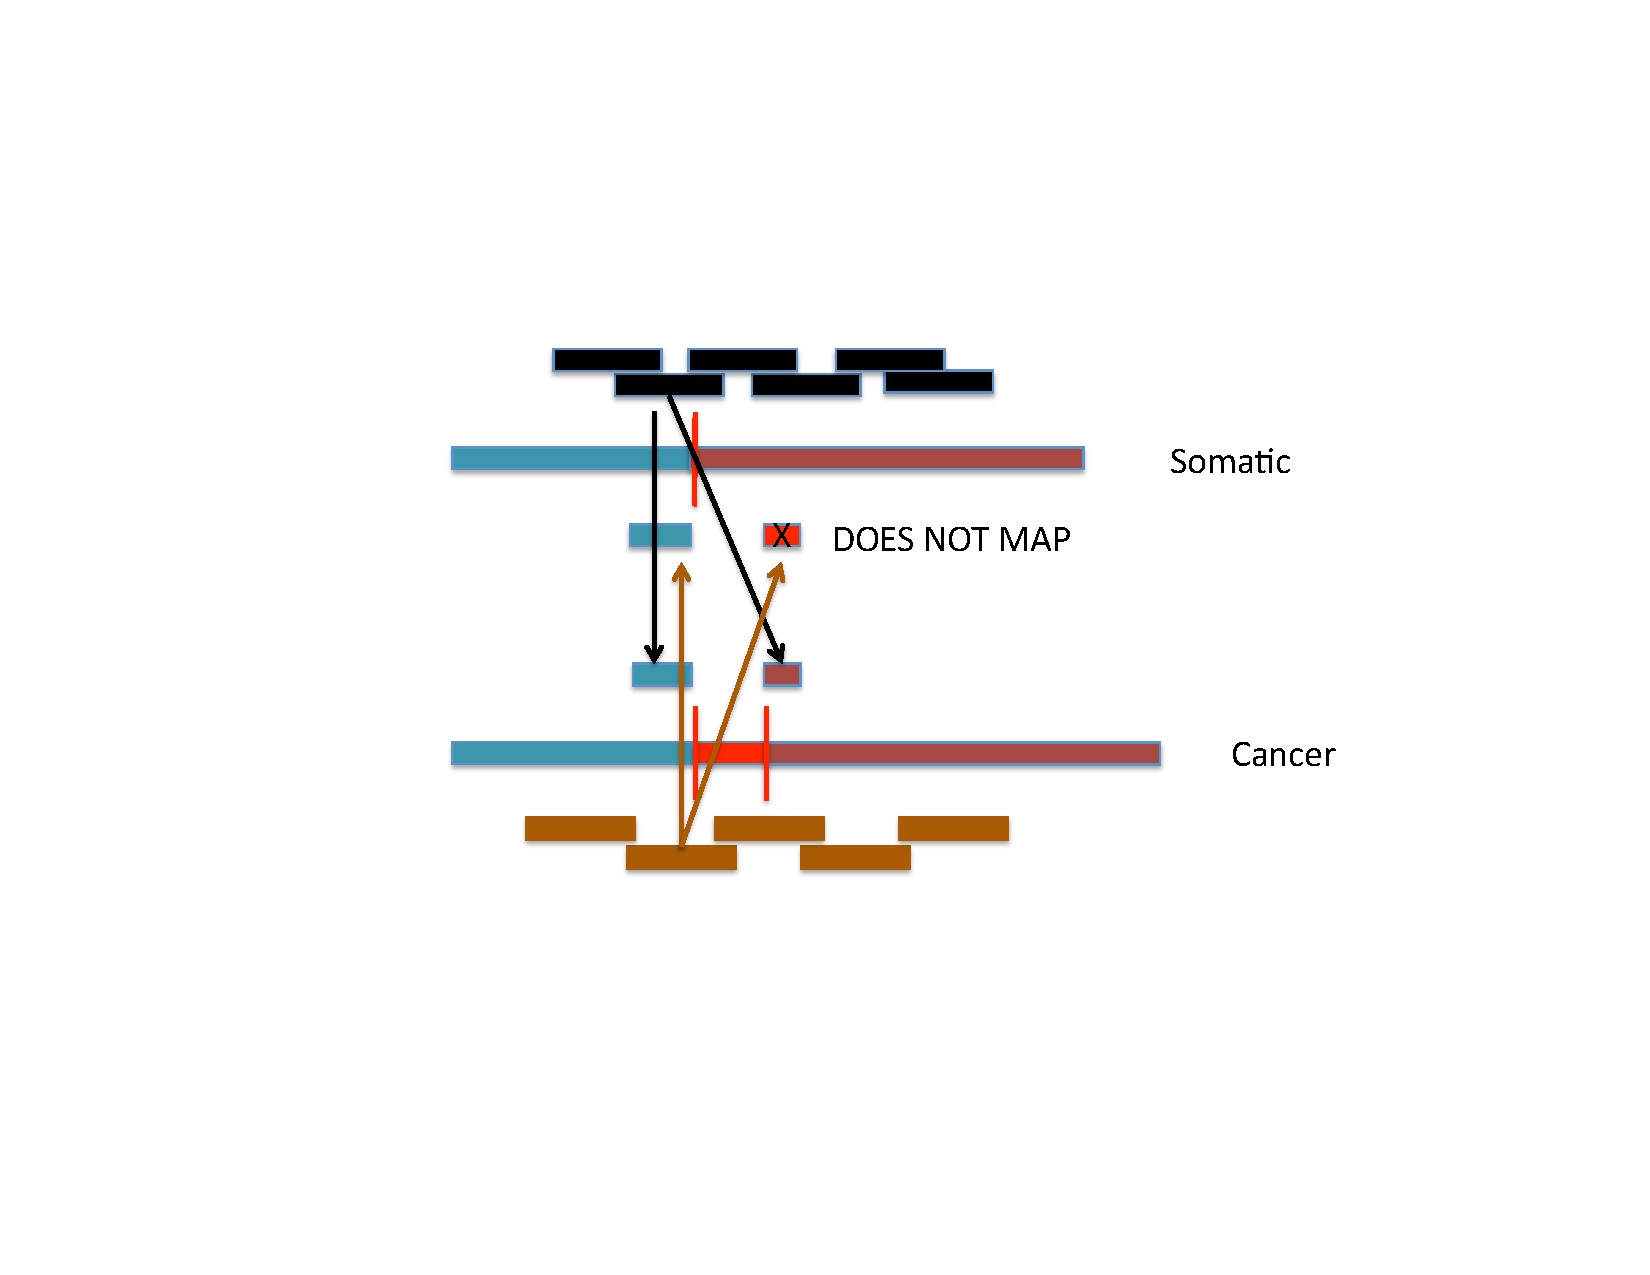
\includegraphics[width = 0.95  \linewidth]{../Code/Figures/DeletionBias.pdf}
\end{center}
\caption{{\bf Deletion bias of unidirectional mapping.} In the case of a novel insertion in the cancer genome, a cancer split-read will only have one part map to the normal, as the novel region does not match anywhere on the genome. However, both parts of a normal split-read will map to the cancer genome, each part flanking the novel insert. Having both parts of the split-read map to the opposing geneme greatly improves the SV discovery rate and confidence.}
\label{fig:DeletionBias}
\end{figure}

\subsection{Direct Somatic/Cancer Comparison}
The proposed method helps overcome the shortcomings of the traditional method primarily by comparing the two genomes directly. 

\begin{figure}[ht]
\centering
\subfigure[Indirect Comparison]{%
	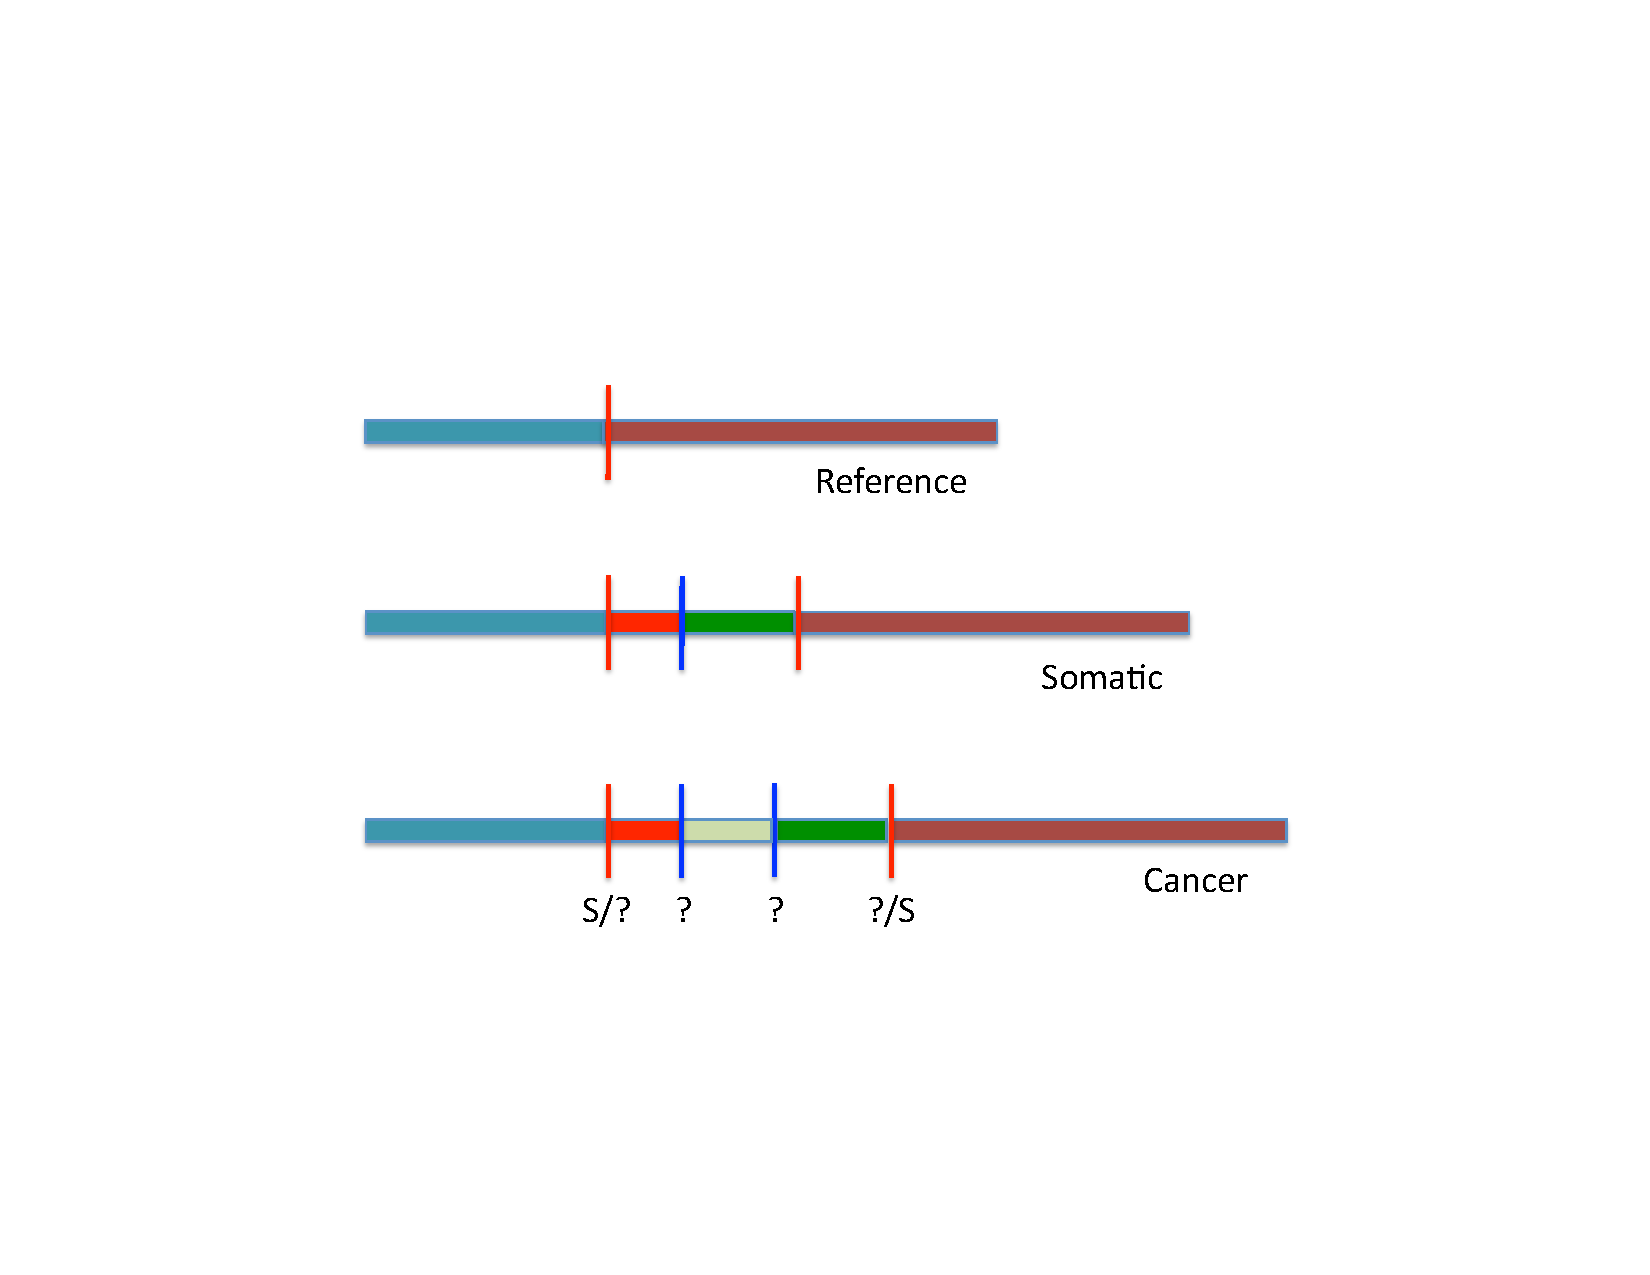
\includegraphics[width = 0.95  \linewidth]{../Code/Figures/InsertionIndirect.pdf}
	\label{fig:InsertionIndirect}}
\quad
\subfigure[Direct Comparison]{%
	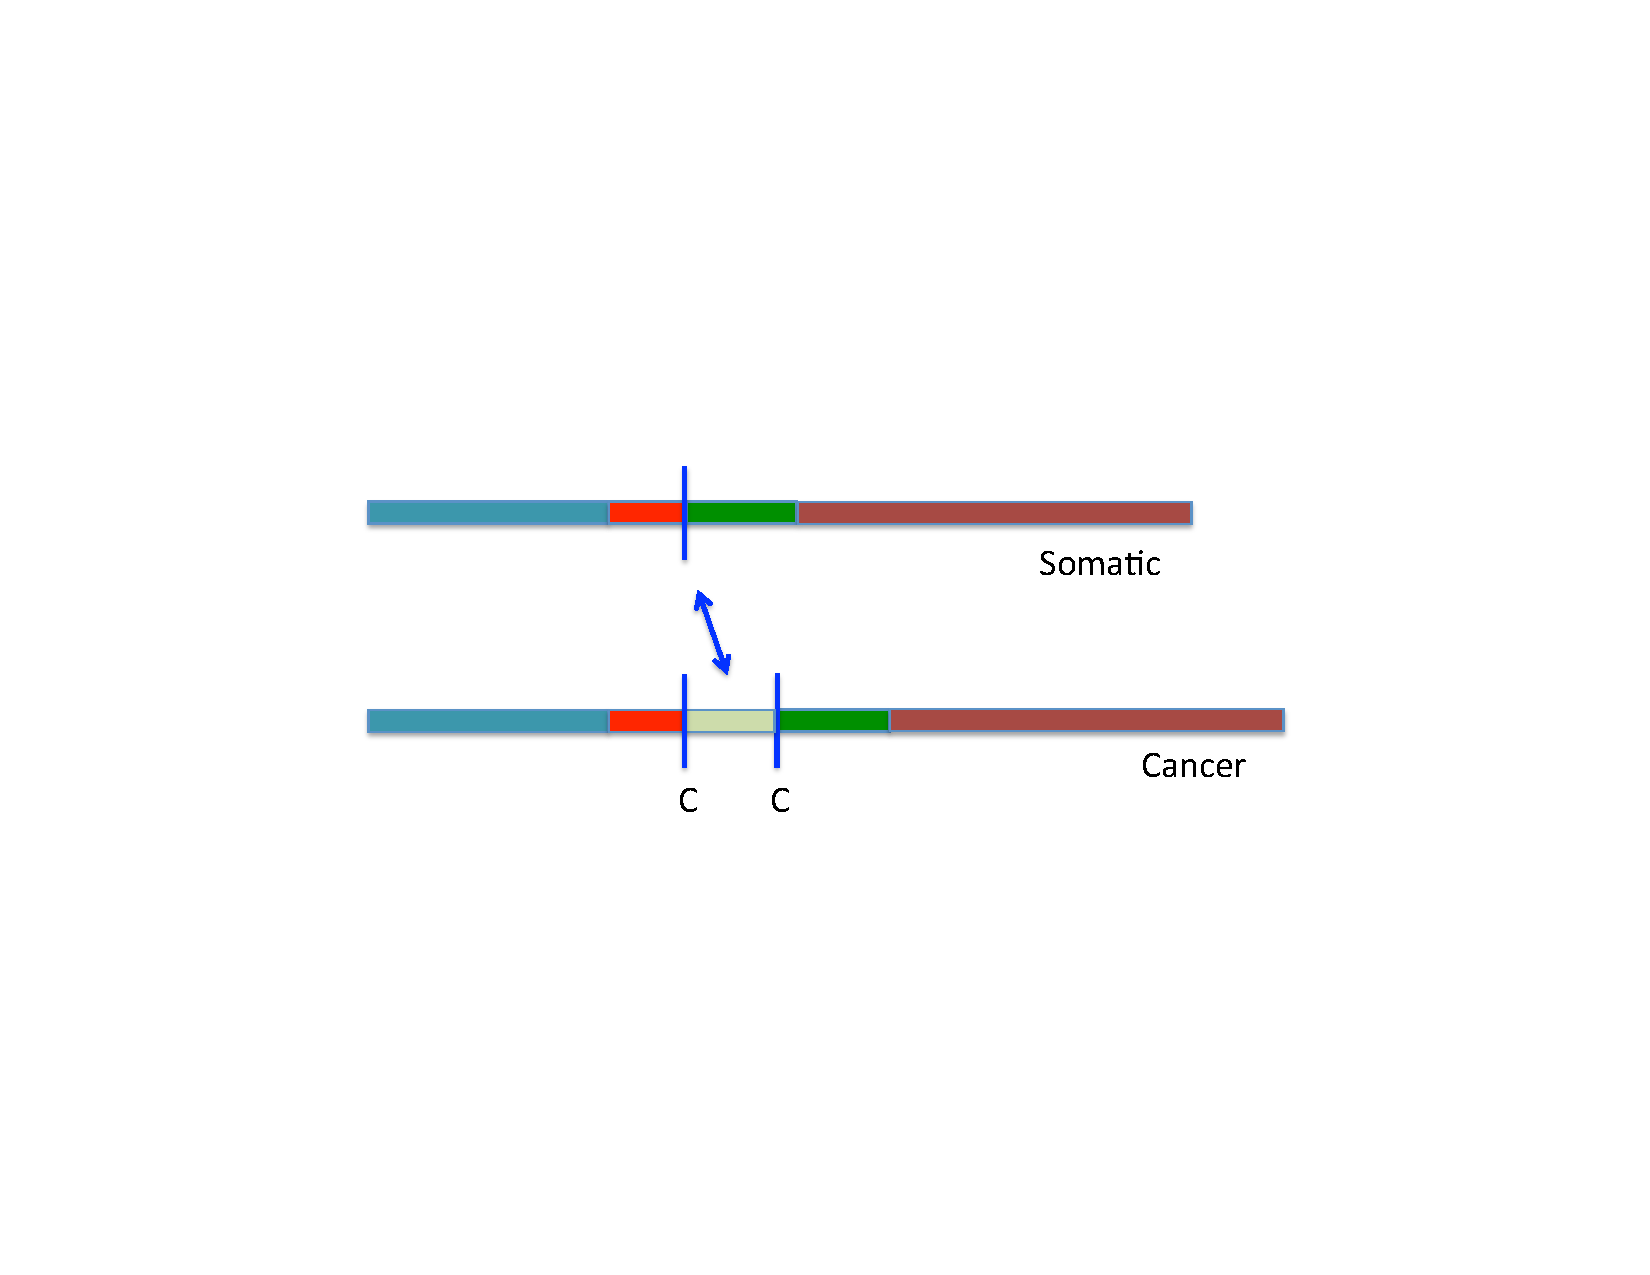
\includegraphics[width = 0.95  \linewidth]{../Code/Figures/InsertionDirect.pdf}
	\label{fig:InsertionDirect}}
%
\caption{{\bf Indirect vs direct comparison of nested insertion.} In the indirect comparison, the entire inner region, whether with or without an additional somatic insertion, is novel and thus only its outer breakpoints are detected. These outer breakpoints, however, are not somatic mutations and are present in both the normal and tumor genomes. Thus the inner breakpoint is overlooked. The direct comparison, in contrast, ignores the outer breakpoints, as they are not different from the normal to cancer genomes (only differ between genomes and reference). It instead only directs the somatic breakpoints, as these differ between the normal and cancer genomes.}
\label{fig:NestedInsertion}
\end{figure}

\begin{figure}[ht]
\centering
\subfigure[Indirect Comparison]{%
	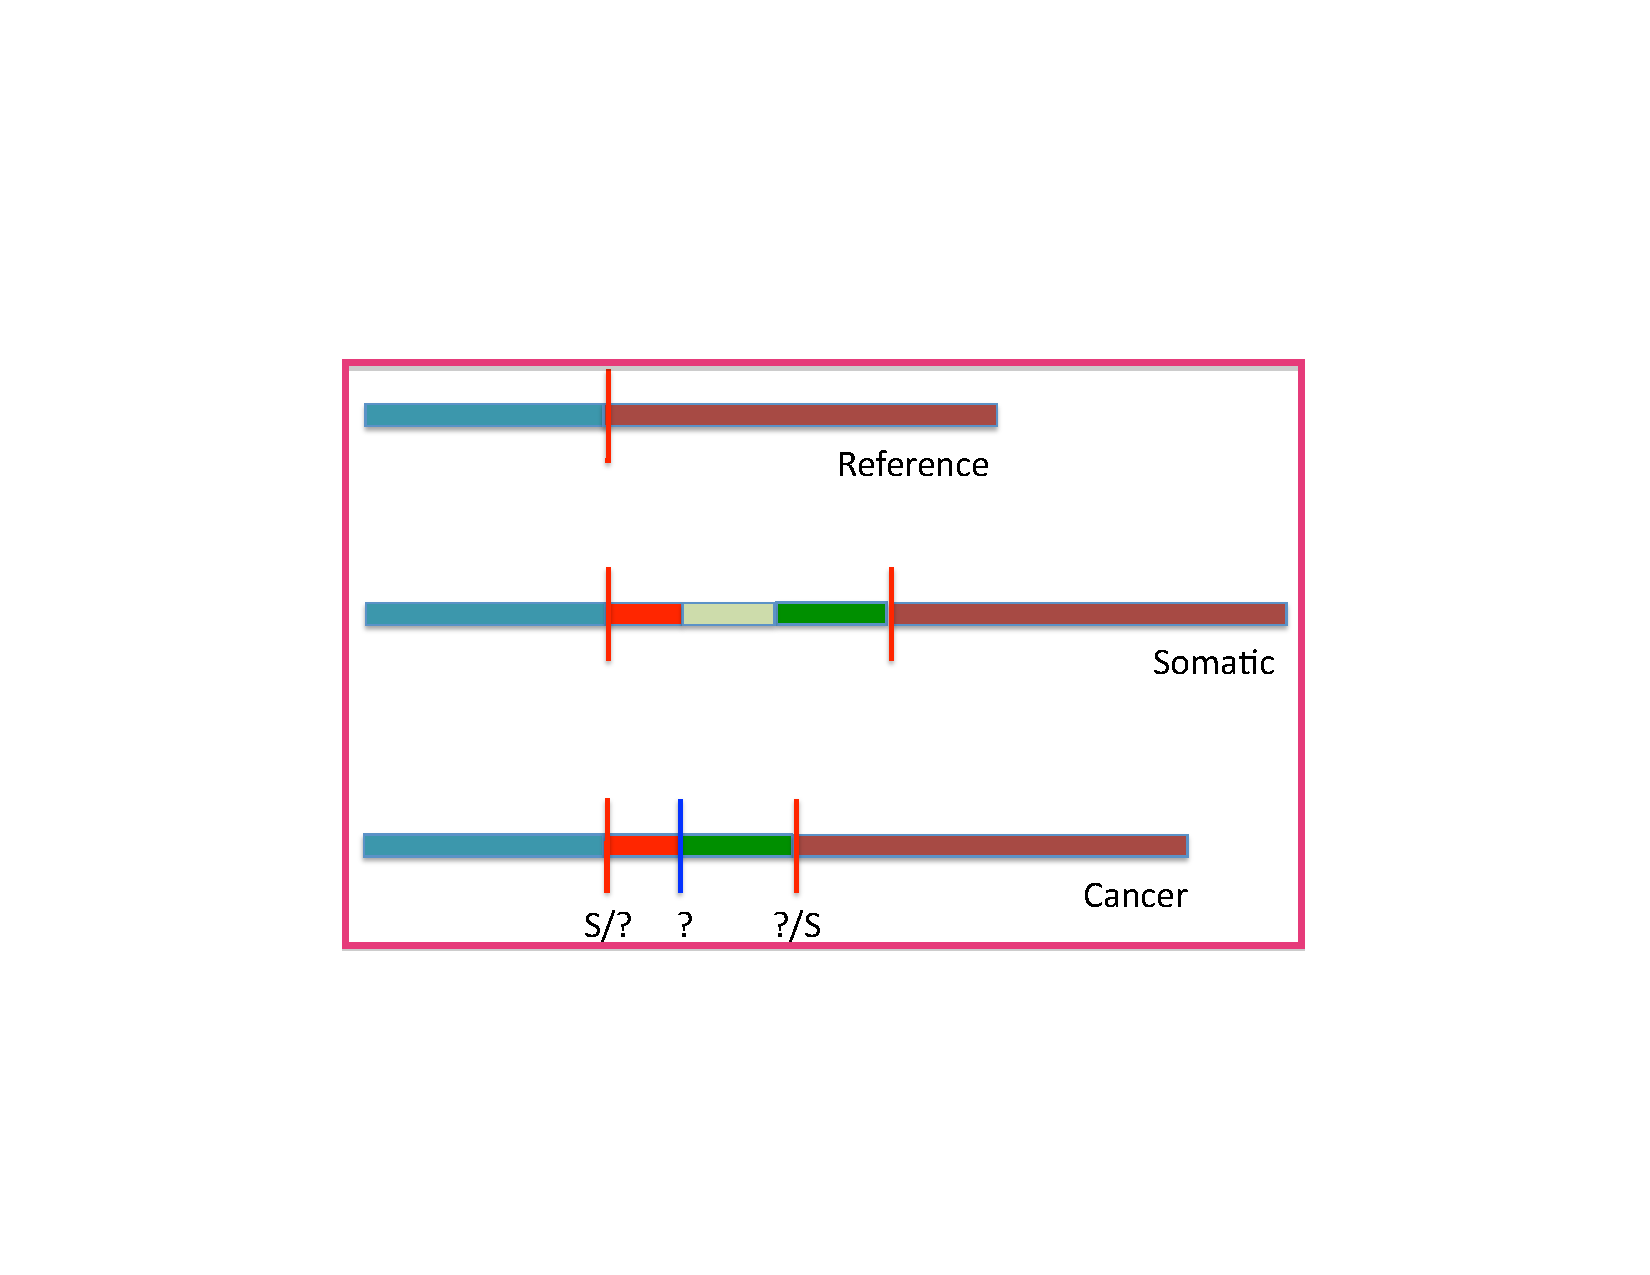
\includegraphics[width = 0.95  \linewidth]{../Code/Figures/DeletionIndirect.pdf}
	\label{fig:DeletionIndirect}}
\quad
\subfigure[Direct Comparison]{%
	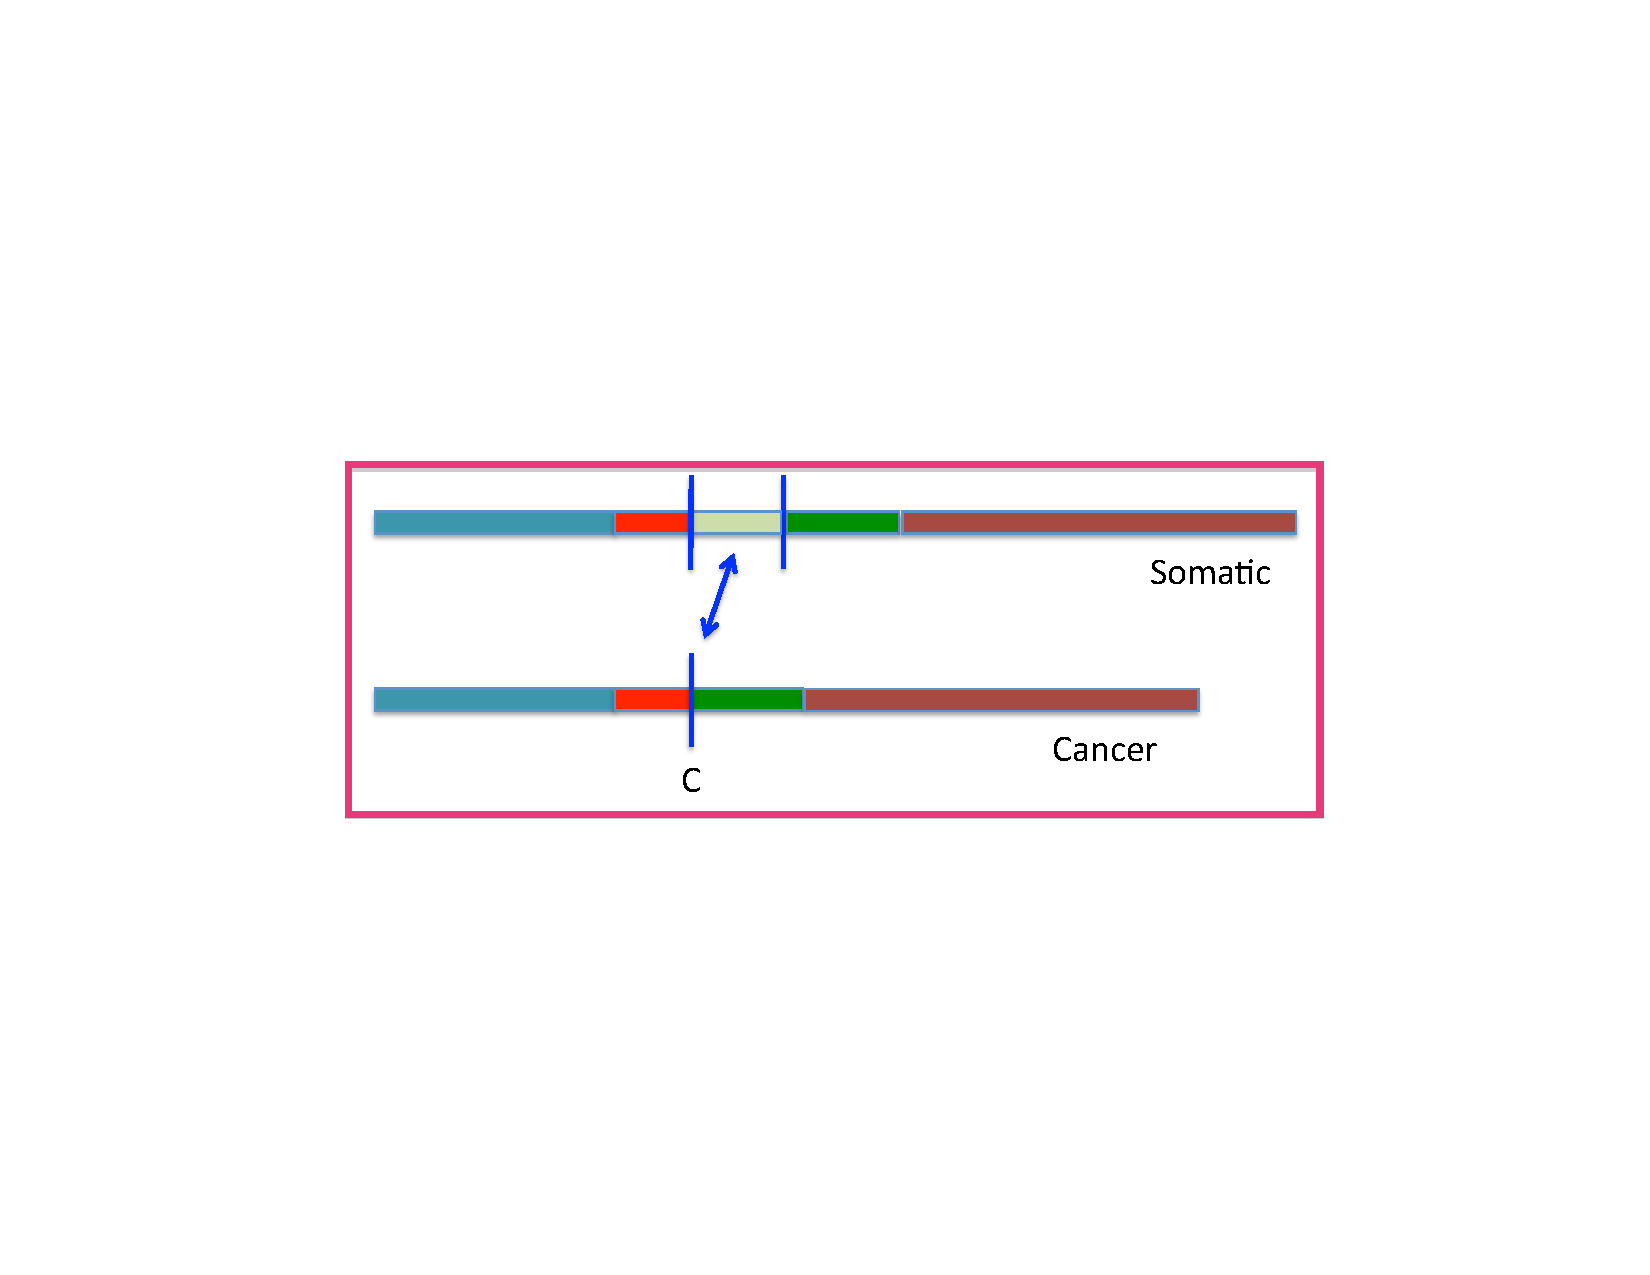
\includegraphics[width = 0.95  \linewidth]{../Code/Figures/DeletionDirect.pdf}
	\label{fig:DeletionDirect}}
%
\caption{{\bf Indirect vs direct comparison of deletion nested in insertion.} In the indirect comparison, the entire inner region, whether with or without an additional somatic deletion, is novel and thus only its outer breakpoints are detected. These outer breakpoints, however, are not somatic mutations and are present in both the normal and tumor genomes. Thus the inner breakpoint is overlooked. The direct comparison, in contrast, ignores the outer breakpoints, as they are not different from the normal to cancer genomes (only differ between genomes and reference). It instead only directs the somatic breakpoints, as these differ between the normal and cancer genomes.}
\label{fig:NestedDeletion}
\end{figure}

\chapter{Materials and Methods}
All code and a list of dependencies is available at https:\slash \slash github.com\slash weincody\slash SVDC.

\section{SV Detection Method}
\subsection{Initial Step-Wise Assemblies}
Because the normal and cancer genomes are being compared directly to one another, the first step in this method is to assemble each genome. Reference-guided assembly is almost essential for a usable assembly of a genome as complex as the human genome. First the normal genome is assembled using the human genome Hg19 as a reference. Next, the tumor reads are assembled using the now assembled normal genome as a reference. Using the normal genome as a reference for the tumor genome minimizes compounding error and the possibility of having false differences between the genomes arise from the assembly step. If there is a mistake in the assembly of the normal genome, for instance, then an independent correct assembly of the cancer genome would incorrectly detect an SV at this position. However, if the cancer genome is assembled using the normal as a reference, this error would likely be propagated to the cancer genome, and while not ideal to have an incorrect assembly, an incorrect breakpoint would not be called. Another reason for this choice is that the tumor genome is actually derived from the normal, so there should be a very high degree of similarity between the two.

\begin{figure}[!ht]
\begin{center}
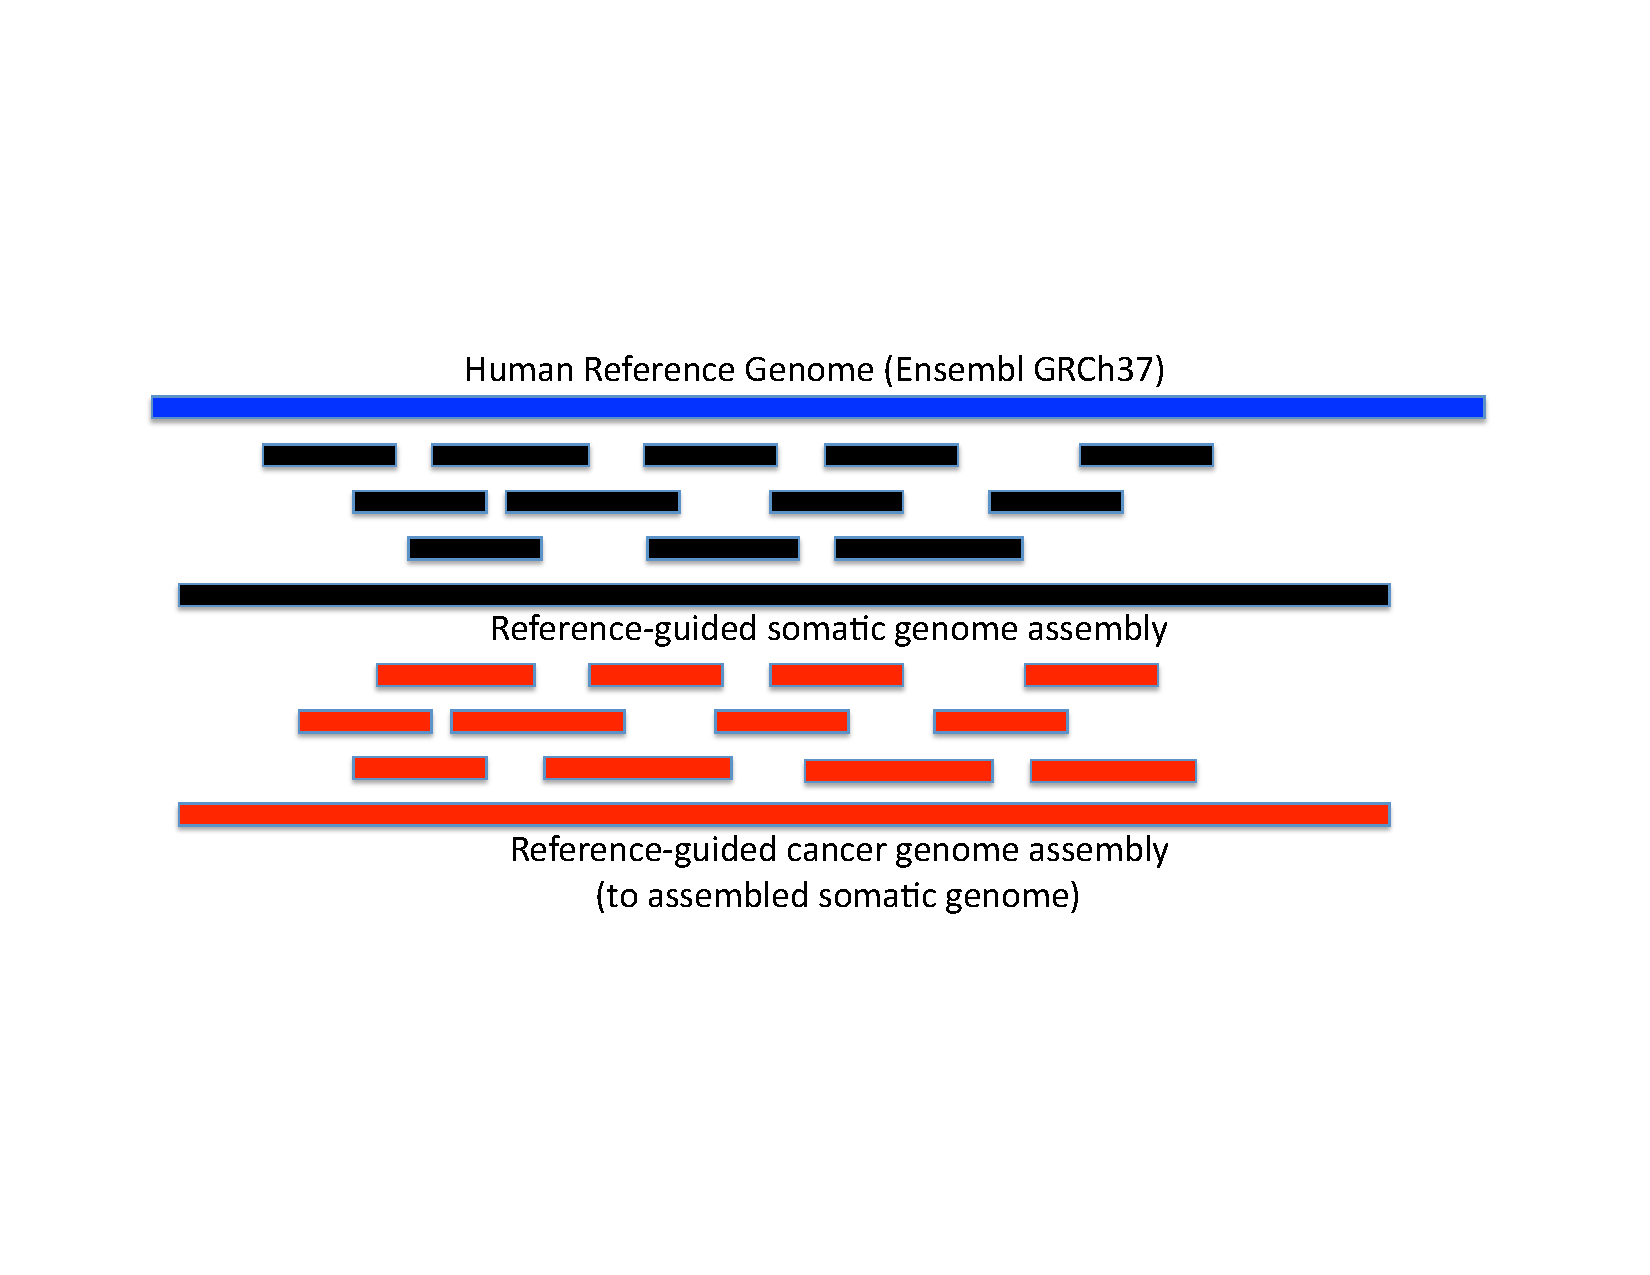
\includegraphics[width = 0.95  \linewidth]{../Code/Figures/RefGuidedAssembly.pdf}
\end{center}
\caption{{\bf Reference-guided assembly.}  The reads from the normal genome are assembled using the human reference genome Hg19 as a reference. Then the tumor reads are in turn assembled using the now assembled normal genome as a reference.}
\label{fig:RefGuidedAssembly}
\end{figure}

\subsection{Alignments}
These reference sequences are first indexed with bowtie2 \cite{langmead2012fast} using the default parameters. This allows for easy referencing once the opposing reads are mapped onto each genome. We then map the raw tumor reads to the assembled normal genome and the normal reads to the assembled tumor genome using bowtie2. The cross-mapping is an essential step for two reasons. First, soft-clipped read SV detection has a bias towards detecting deletions rather than insertions. This is because when we map a read from a deletion, each side of the read should partially map to a region flanking the deleted region on the reference sequence. When both sides partially map, we can call this event with higher confidence. In a novel insertion, however, only the non-novel region can map to the reference, reducing confidence in half and greatly reducing our discovery rate. When we map in both directions, we should ideally detect both the insertion event on one genome and the deletion on the other. This provides us with two possible situations: either only one event, the insertion or more likely the deletion, is detected. In this case, we either have a false positive or false negative, as where there is an indel in one genome there must also be the oppoiste in the other genome. Because insertions are difficult to detect, we may indeed pick up some novel indel events as singular deletion events in one genome that would otherwise be missed checking for an insertion in one direction. Our first output is these singular events as a list of potential SVs that may be missed with traditional methods that only map reads in one direction, and expect to recover some number of novel insertion events missed by the deletion bias.

\begin{figure}[!ht]
\begin{center}
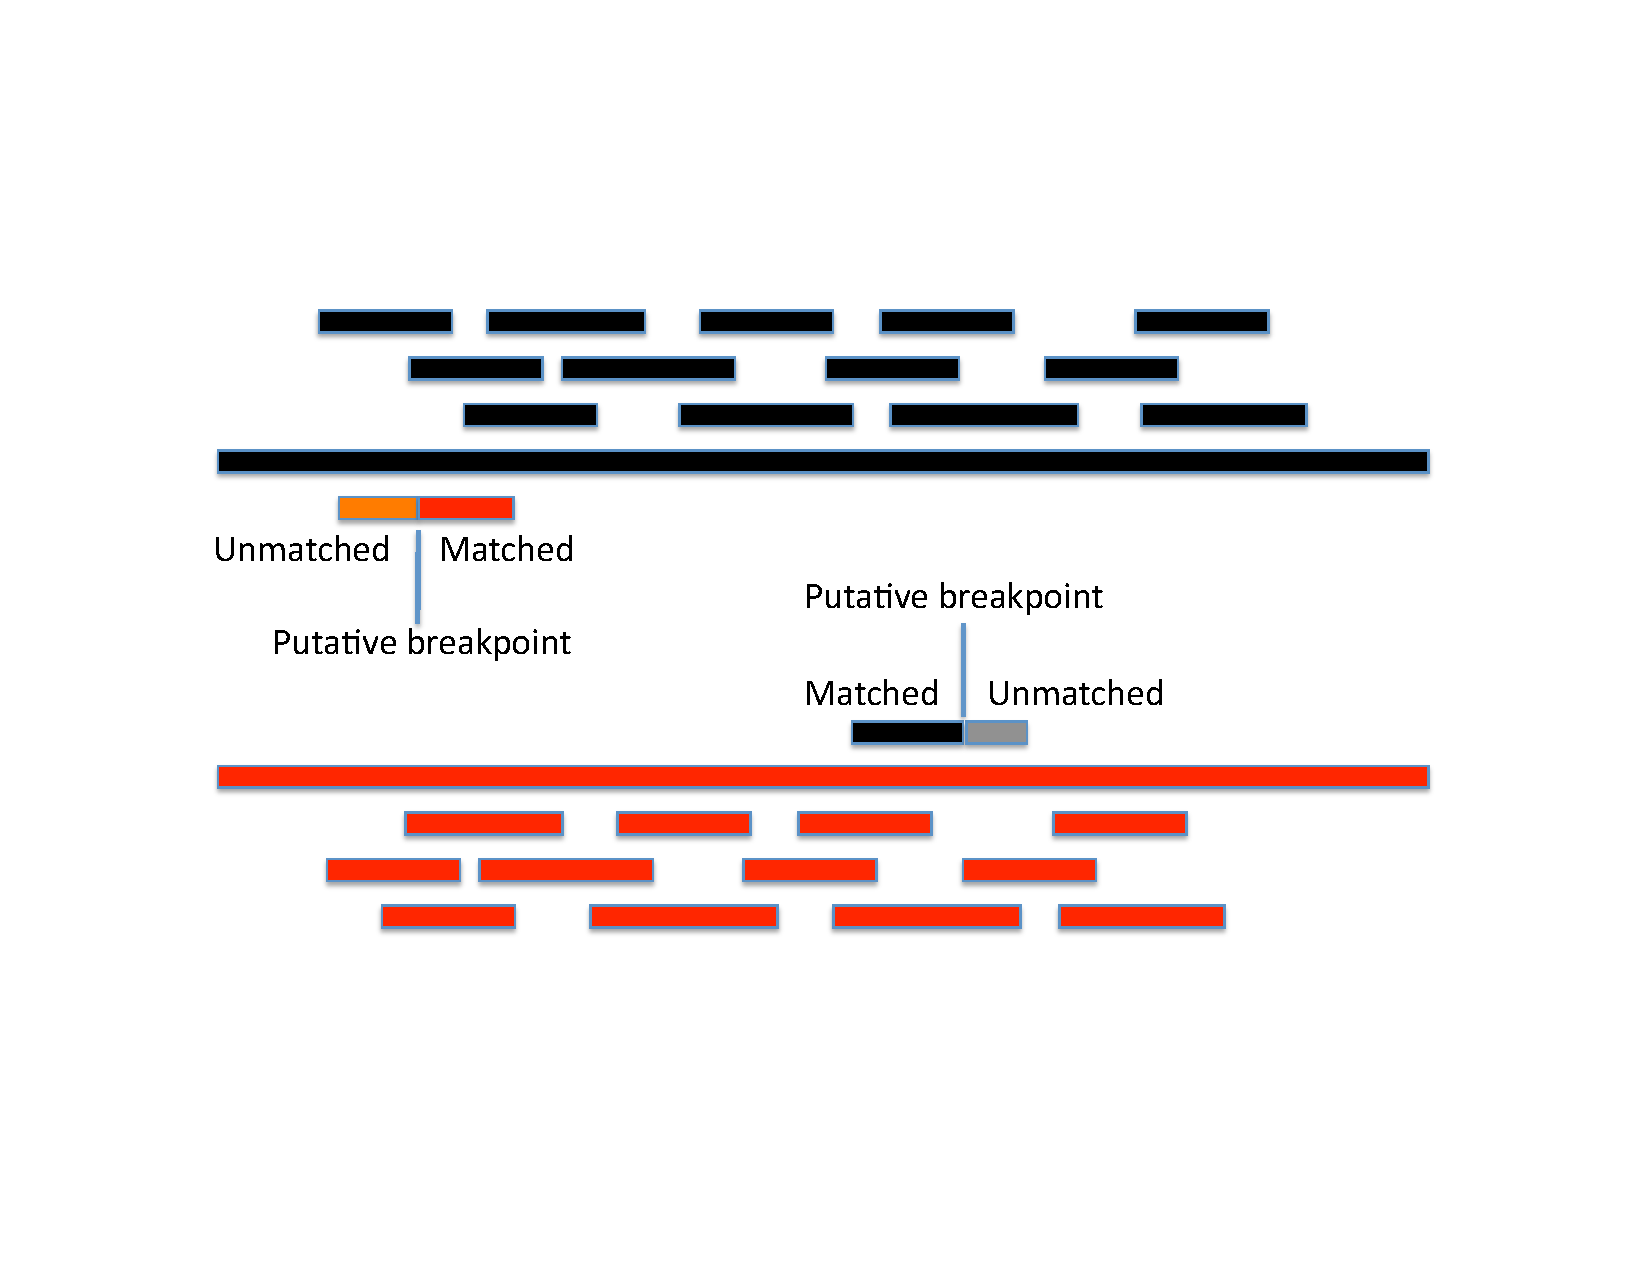
\includegraphics[width = 0.95  \linewidth]{../Code/Figures/SplitReadMapping.pdf}
\end{center}
\caption{{\bf Split-read mapping.}  When a read only partially maps to the opposing genome, the position at which there is no longer a match provides a putitive breakpoint for an SV in this position. We map normal reads to the tumor genome and tumor reads to the normal genome and compare split reads from both, as all true SVs should be detected on both genomes.}
\label{fig:SplitReadMapping}
\end{figure}

Our second output is a list of events that are detected in both genomes, which gives us higher confidence that they are true events. This is especially helpful for split-read detection, as it generally has a high false positive rate for breakpoint calling \cite{abel2013detection}. Having a list of high confidence breakpoints is a very helpful tool when wanting to extend the analyses further. Confirming breakpoints with Sanger sequencing is a common technique, but due to the high monetary and temporal cost of local sequencing, a small subset of the breakpoints is generally used \cite{jiang2012prism}. Thus only the most promising breakpoints should be chosen. This output would provide a solid initial subset for further sequencing and analyses.

Pindel and PRISM only perform with 26.3-37.6\% recall on real data for indels 21-100bp in length \cite{jiang2012prism}, demonstrating the need for higher accuracy provided with the first, single-hit output. Further, both of these methods had extremely low precision, $<$4\%, on indels 51-100 bp \cite{jiang2012prism}, showing a great need for a refined list of breakpoints, which is provided in the second, dual-hit output.

\subsection{SV Calling}
Samtools is used to convert the bowtie2 SAM output file into BAM format. The normal-to-tumor and tumor-to-normal alignment files are then each used as an input for Socrates to call breakpoints. Socrates uses the soft-clipped alignments to generate two lists of predicted breakpoints. Every breakpoint can have reads mapped to either side of it, and having reads mapped to both sides gives a much higher confidence for a correct call at that breakpoint. Thus we ignore the output of unpaired breakpoints and use the paired breakpoints output, which contains all breakpoints that had reciprocal support from each side. 

From this Socrates paired output, a custom java program extracts, parses, and outputs the sequences flanking either side of each breakpoint into a FASTA file. These are then prepared for cross-checking for matches on each genome by indexing each FASTA file with bowtie2. To check for matching events between genomes, each FASTA file of flanking regions is mapped to the opposing indexed FASTA file using bowtie2 (we check both directions in case of a length difference, in which case the shorter may be mapped to the longer but not vice versa).

We then use another java program to determine which breakpoints correspond. There is a correspondence if 1) flanking regions from a given breakpoint in the cancer genome map to a breakpoint in the normal genome and 2) flanking regions from that same breakpoint in the normal genome map back onto the breakpoint in the cancer genome.

This system of comparing flanking regions to identify correpsonding breakpoints is based upon the property that every breakpoint should have at least one flanking side conserved between the original and derived genomes.

\begin{figure}[!ht]
\begin{center}
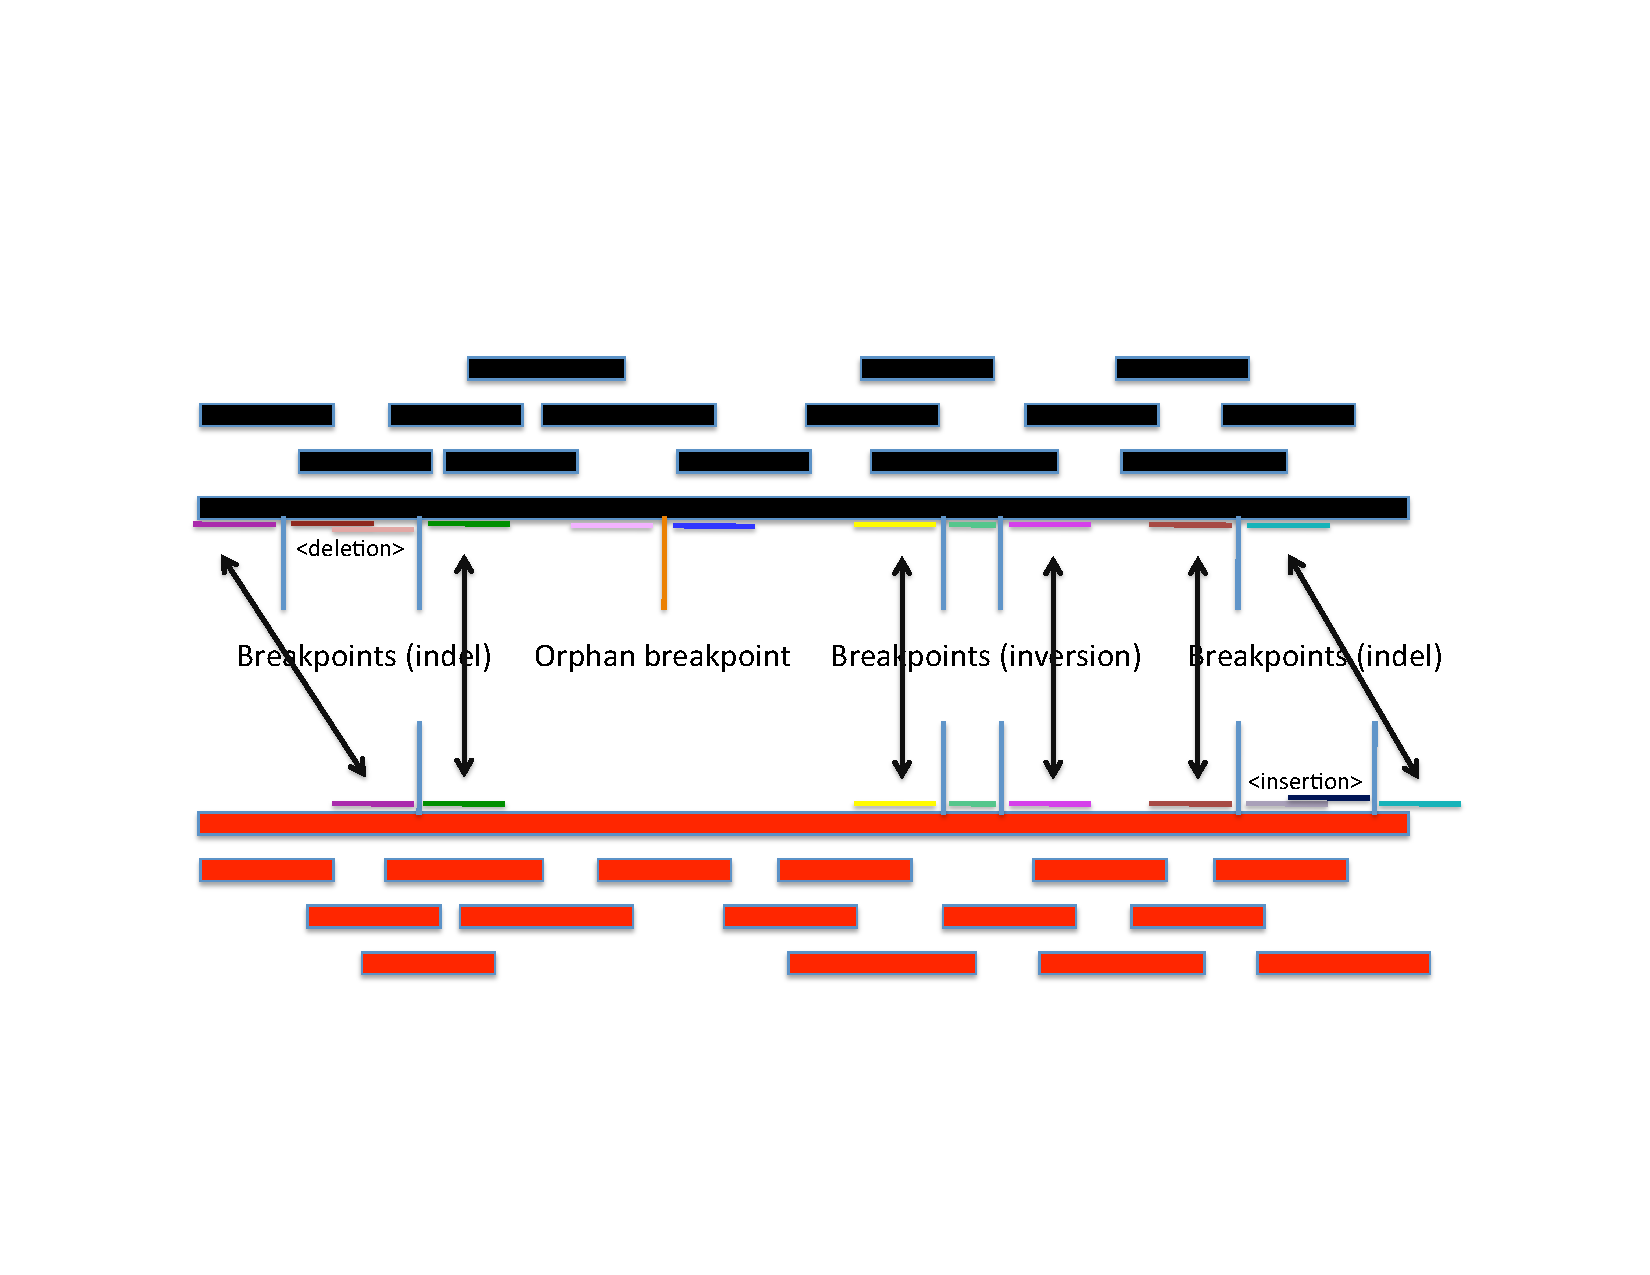
\includegraphics[width = 0.95  \linewidth]{../Code/Figures/FlankConservation.pdf}
\end{center}
\caption{{\bf Conservation of sequences flanking breakpoints.} In any type of SV, the region just beyond the breakpoint is unaffected and thus conserved between the original and derived genomes. Note that the orphan breakpoint would be on the first output list (detected in one direction), while those that map to a corresponding breakpoint would be on the second output list (detected in both directions).}
\label{fig:FlankConservation}
\end{figure}

\subsection{SV Annotation}
Annotations from the breakpoint detectors, if available as a feature of that software, can be preserved with the pipeline. If there is no annotation, the region can be blasted, as the sequence is available on the output genomes, and the function of this region will be inferred for some number of breakpoints. The results from the low confidence (one direction mapped) and high confidence (both directions mapped) outputs will be compared.]

\section{Ideal Assembly}

\subsection{Simulate SVs}
I wrote a script in \texttt{Python 2} to simulate SVs in a chromosome (code available at https:\slash \slash github.com\slash weincody\slash SVDC). The inputs are the file name of the original sequence; the name of the sequence to be output; and the number of events to be simulated, which we call $N$. To generate the location of the start of the first SV event, the length of the chromosome is divided by $N$ and a location between 0 and $L/N$ is chosen. An event type is then chosen, all equally probable, with possibilities being a novel insertion, deletion, inversion, or translocation. The randomly selected event then occurs at the chosen position. $L$ is then updated after the first event, and the start location of the second event is then chosen randomly between $L/N$ and $2*(L/N)$. An event type is again randomly chosen from a uniform distribution, occurs at the start location, $L$ is updated, and the next event occurs between the next segment of length $L/N$. This occurs N number of times.

Insertions were simulated by drawing a random integer for its length, $L$, between 1 and 10,000. Then a sequence is generated by selecting a base, chosen randomly from "G", "C", "A", or "T", $L$ number of times and concatenating these into the novel insert. 

Deletions and inversion were simulated similarly, with a region of length $L$ between 1 and 10,000 to be removed and inverted, respectively.

When a translocation was called, the initial region is subject to the deletion. Then a location is chosen randomly throughout the entire genome for the region to be reinserted.

The outputs are the simulated genomes, a matrix of indices corresponding to each generated genome and the original index in the reference genome, and a matrix of events that tracks the history of the simulated mutations through time and has a corresponding index for each genome in the index matrix.

This script was then run on the first 1/100th bases of a cleaned Hg19 chromosome 11, e.g. all large continuous regions of Ns removed, with the number of events set to 15 to generate our "normal genome," a simulated population variant from the reference. The script was then run again on this simulated chromosome with the number of events set to 20 to generate a "tumor genome" derived from the normal genome.

\subsection{Ideal Analysis}
I investigated how the direct comparison method compares to Socrates, the breakpoint detector from which it is adapted from, under the most ideal, error-free conditions, as a proof of concept and to reveal a maximum potential of the method as assemblers improve. A simulation for each of the key features of the method, detecting nested SVs and improving the deletion bias, was constructed. 

To perform the first analysis testing nested SVs, data was generated with no errors in the reads and a correct assembly given. A novel insertion occurred from Hg19 to the "normal" genome, and then a subsequent event, which could be either an insertion, deletion, or inversion with equal probability, occurred within the novel insertion. This was repeated $N = 15$ times, with each subsequent iteration occurring downstream of the previous.

To perform the second analysis testing deletion bias, the same assumptions were made as in the first with two main differences; there was no restriction on events occuring within a novel region, and translocations were also included. The "normal" reference genome was generated from running the SV simulation script on the Hg19 human chromosome 11. The "cancer" reference genome was then built from running the same script on the "normal" genome. Then from these two reference genomes, reads were generated with 0\% error from the DWGSIM software. The direct comparison pipeline was then run on the resulting reads and reference genomes. The simulation also assumes that the true genome assemblies are known, serving as a proof of concept under the best possible circumstances. The pipeline was then compared with the standard implementation of Socrates, which only utilizes raw reads and the reference genome. The Socrates annotate feature with the --normal flag was used to generate the list of somatic mutations for comparison. Note that both the DC pipeline and Socrates only utilized the paired output from Socrates in this comparison.

Statistical analyses of the results were performed in \texttt{R}.

\chapter{Results}

Two simulations were performed to demonstrate the ability to 1) resolve the deletion bias and 2) detect nested SVs. The first simulation also acts as a test of general performance, as they are simply random SVs.

\section{Deletion Bias (Regular Events) Simulations}

The first simulations were designed to test general performance and ability to resolve the deletion bias found in the traditional method.

\begin{table}[h]
\begin{center}
\begin{tabular}{|c|c|c|c|c|c|}\hline
         & Insertion & Deletion & Inversion & Translocation & FP \\
        \hline 
        Actual Event Count & 36 (144) & 29 (116) & 42 (168) & 43 (344) & -\\
        \hline 
        DC Matched BPs & 1 & 2 & 1 & 226 & 72\\
        \hline 
        DC Unmatched BPs & 30 & 24 & 4 & 68 & 156\\
        \hline 
        Socrates BPs & 0 & 24 & 3 & 126 & 226\\
        \hline
\end{tabular}
\caption{{\bf Performance comparisons on simulated data set.} Data is summed across 10 simulations. DC represents the direct comparison method when the ideal assemblies were supposed as known. The value listed is the total number of hits for that output in that category - a hit represents correctly calling a breakpoint for a type of SV. A false positive is a called breakpoint that did not actually occur. The value in parentheses for actual event counts denotes the number of breakpoints generated from the events in that category.}
\end{center}
\end{table}

The results show that the DC method (combined matched and unmatched outputs) is able to detect 31 breakpoints, giving a mean sensitivity of 0.226, while Socrates did not detect any. This demonstrates both the deletion bias as being very present in the traditional method and that direct comparison can provide a way to eradicate this.

The DC method actually outperformed Socrates alone in every SV class in both sensitivity, which is defined as $(true\ positives) / (events)$, and false discovery rate (FDR), defined as $(false\ positives) / (true\ positives + false\ positives)$. 

\section{Nested Events Simulations}

The second set of simulations were designed to test the ability of the DC method to detect events nested within regions not present on the reference sequence. Novel regions were added to the reference (subset of Hg19 chromosome 11) to obtain the "normal" genome, and subsequent events were added within the bounds of these novel regions to obtain the "tumor" genome, derived from the normal. The DC pipeline and Socrates alone were both run on the resulting genomes, and performance of the DC matched output, DC unmatched output, and Socrates alone output were compared (Table 3.1).

\begin{table}[h]
\begin{center}
\begin{tabular}{|c|c|c|c|c|}\hline
         & Nested Insertion & Nested Deletion & Nested Inversion & FP \\
        \hline 
        Actual Event Count & 49 (196) & 47 (188) & 54 (216) & -\\
        \hline 
        DC BPs & 49 & 51 & 13 & 221 \\
        \hline
        Socrates BPs & 0 & 0 & 0 & 103 \\
        \hline
\end{tabular}
\caption{{\bf Performance comparisons on simulated data set with nested SVs.} Data is averaged across 10 simulations. All somatic mutations occured within a novel normal region. In theory, all non-DC methods should miss these events and make no somatic mutation predictions. The DC method should be able to detect these events. The value listed is the total number of hits for that output in that category - a hit represents correctly calling a breakpoint for a type of SV. A false positive is a called breakpoint that did not actually occur. The value in parentheses for actual event counts denotes the number of breakpoints generated from the events in that category.}
\end{center}
\end{table}

The results show that while 

\chapter{Discussion}
\section{Applications of this pipeline}
[Will discuss the succusses and failures of each of the two outputs in the simulations:
	1) Did the first output provide us with additional, true breakpoints?\\
	2) Did the second output have a higher hit rate and lower false positive rate?\\
Was there less of a bias towards deletions in the DC method with the number of predicted indels?]

[Results pending: The simulations show the lack of ability for standard methods to detect any SVs within a novel region, which in some sense we couldn't have known what we are missing. The concept of direct comparison has the potential to resolve this issue, as we see most of these events are called when comparing directly. We expect these events to be fairly common, as there is much population level variation among humans, and rare variants are increasingly being found to play a role in genetic disease prevalence.

We also see from the ideal results that there is a deletion bias in the traditional methods and also that bidirectional mapping has the potential to drastically reduce this bias. However, the limiting step in this method in particular is the reliance upon an initial assembly, which reduced the accuracy of all SV calls.]

This method is not desigend to replace other methods for detecting SVs, but primarily to fill in the gap of novel insertions and nested SVs that would likely otherwise go unnoticed. Thus this method would be best used in supplement with methods that do not rely on assemblies and can find majority of the easier-detected deletions, smaller indels, SNPs, etc. But as sequencing read lengths grow and assembly tools become more accurate, using these tools with a direct comparison approach will become more powerful and a personalized genome more useful and accurate, while the traditional approach can only improve with read length and cannot provide more information than a list of breakpoints.

\section{Future directions}
This pipeline can be used with any reference-guided assembler and breakpoint detector, so it will improve with advances in these tools. As assembly is a huge limiting step in this pipeline, the next step would be to modify the pipeline to compare reads directly rather than first making draft assemblies. Another option would be to adapt the assembly in progress by using the predicted breakpoints. SHEAR \cite{landman2014shear} uses such a back-and-forth breakpoint predictor/assembler, but this specific tool still compares reads indirectly to the reference.

As other methods shift towards providing a full, personalized genome, the standard for SV annotation should shift from being anchored to location on a reference to relying solely on sequence look-up. It is almost counter-intuitive to reference 2 different locations in 2 genomes by a third different location in the reference sequence when all 3 share common sequence, and this is actually inhibitory when technology allows us to move further away from reliance on a single reference genome. Both a shift towards sequence-lookup or the above suggested change to direct read comparison would help resolve the issue encountered with this specific method of manual annotation.

Though the technology may not yet be at a place where this implementation of the method is more advantageous than the standard indirect comparison SV detectors, the largely overlooked limitations of indirect comparison, namely deletion bias and failure to detect nested SVs, are brought to light here; further, a general method, direct bi-directional mapping, is offered to overcome both of these. While the traditional methods encounter these issues at a fundamental level and will remain stagnant to them regardless of technological advances, this method should improve with both sequencing and assembling technology, offering a potential avenue for future SV detection.

%
% Appendices
%
\appendix
\chapter{Simulations}
The simulations were run in \texttt{Python 2}. The algorithm takes an input FASTA file as the reference genome and a number of events, $N_E$. Then for

\begin{table}[h]
\begin{center}
\begin{tabular}{|c|c|c|c|c|c|}\hline
         & Insertion & Deletion & Inversion & FP \\
        \hline 
        Actual Event Count 1 & 4 (16) & 4 (16) & 7 (28) & -\\
        DC Matched BPs 1 & 0 & 0 & 4 & 4\\
        DC Unmatched BPs 1 & 4 & 4 & 1 & 10\\
        Socrates BPs 1 & 0 & 0 & 0 & 9\\
        \hline 
        Actual Event Count 2 & 7 (28) & 2 (8) & 6 (24) & -\\
        DC Matched BPs 2 & 0 & 0 & 0 & 6\\
        DC Unmatched BPs 2 & 7 & 2 & 0 & 11\\
        Socrates BPs 2 & 0 & 0 & 0 & 6\\
        \hline 
        Actual Event Count 3 & 2 (8) & 5 (20) & 8 (32) & -\\
        DC Matched BPs 3 & 0 & 0 & 2 & 11\\
        DC Unmatched BPs 3 & 2 & 5 & 0 & 18\\
        Socrates BPs 3 & 0 & 0 & 0 & 11\\
        \hline 
        Actual Event Count 4 & 6 (24) & 5 (20) & 4 (16) & -\\
        DC Matched BPs 4 & 0 & 1 & 0 & 12\\
        DC Unmatched BPs 4 & 6 & 5 & 0 & 18\\
        Socrates BPs 4 & 0 & 0 & 0 & 15\\
        \hline 
        Actual Event Count 5 & 3 (12) & 6 (24) & 6 (24) & -\\
        DC Matched BPs 5 & 0 & 3 & 2 & 8\\
        DC Unmatched BPs 5 & 3 & 6 & 0 & 15\\
        Socrates BPs 5 & 0 & 0 & 0 & 15\\
         \hline 
        Actual Event Count 6 & 5 (20) & 4 (16) & 6 (24) & -\\
        DC Matched BPs 6 & 0 & 0 & 2 & 7\\
        DC Unmatched BPs 6 & 5 & 4 & 0 & 23\\
        Socrates BPs 6 & 0 & 0 & 0 & 15\\
         \hline 
        Actual Event Count 7 & 8 (32) & 4 (16) & 3 (12) & -\\
        DC Matched BPs 7 & 0 & 0 & 0 & 4\\
        DC Unmatched BPs 7 & 8 & 4 & 0 & 12\\
        Socrates BPs 7 & 0 & 0 & 0 & 7\\
         \hline 
        Actual Event Count 8 & 3 (12) & 6 (24) & 6 (24) & -\\
        DC Matched BPs 8 & 0 & 0 & 0 & 5\\
        DC Unmatched BPs 8 & 3 & 6 & 0 & 11\\
        Socrates BPs 8 & 0 & 0 & 0 & 6\\
         \hline 
        Actual Event Count 9 & 4 (16) & 6 (24) & 5 (20) & -\\
        DC Matched BPs 9 & 0 & 0 & 2 & 8\\
        DC Unmatched BPs 9 & 4 & 6 & 0 & 19\\
        Socrates BPs 9 & 0 & 0 & 0 & 11\\
         \hline 
        Actual Event Count 10 & 7 (28) & 5 (20) & 3 (12) & -\\
        DC Matched BPs 10 & 0 & 0 & 0 & 7\\
        DC Unmatched BPs 10 & 7 & 5 & 0 & 12\\
        Socrates BPs 10 & 0 & 0 & 0 & 8\\        
        \hline
\end{tabular}
\caption{{\bf Results of deletion bias (regular events) simulations.} Data is for 10 simulations. DC represents the direct comparison method when the ideal assemblies were supposed as known. The value listed is the number of hits for that output in that category - a hit represents correctly calling a breakpoint for a type of SV. A false positive is a called breakpoint that did not actually occur. The value in parentheses for actual event counts denotes the number of breakpoints generated from the events in that category.}
\end{center}
\end{table}

\begin{table}[h]
\begin{center}
\begin{tabular}{|c|c|c|c|c|c|}\hline
         & Insertion & Deletion & Translocation & Inversion & FP \\
        \hline 
        Actual Event Count 1 & 7 (28) & 0 (0) & 6 (48) & 2 (8) & -\\
        DC Matched BPs 1 & 0 & 0 & 9 & 0 & 3\\
        DC Unmatched BPs 1 & 6 & 0 & 4 & 0 & 9\\
        Socrates BPs 1 & 0 & 0 & 5 & 0 & 15\\
        \hline 
        Actual Event Count 2 & 2 (8) & 4 (16) & 5 (40) & 4 (16) & -\\
        DC Matched BPs 2 & 0 & 0 & 21 & 0 & 3\\
        DC Unmatched BPs 2 & 2 & 4 & 7 & 0 & 10\\
        Socrates BPs 2 & 0 & 4 & 15 & 0 & 26\\
        \hline 
        Actual Event Count 3 & 2 (8) & 2 (8) & 8 (64) & 3 (12) & -\\
        DC Matched BPs 3 & 0 & 0 & 41 & 1 & 14\\
        DC Unmatched BPs 3 & 2 & 1 & 12 & 1 & 28\\
        Socrates BPs 3 & 0 & 1 & 20 & 1 & 15\\
        \hline 
        Actual Event Count 4 & 5 (20) & 4 (16) & 0 (0) & 6 (24) & -\\
        DC Matched BPs 4 & 0 & 0 & 0 & 0 & 46\\
        DC Unmatched BPs 0 & 0 & 0 & 0 & 0 & 44\\
        Socrates BPs 4 & 0 & 0 & 0 & 0 & 37\\
        \hline 
        Actual Event Count 5 & 3 (12) & 3 (12) & 3 (24) & 6 (24) & -\\
        DC Matched BPs 5 & 0 & 0 & 16 & 0 & 6\\
        DC Unmatched BPs 5 & 3 & 3 & 7 & 2 & 14\\
        Socrates BPs 5 & 0 & 3 & 9 & 0 & 26\\
         \hline 
        Actual Event Count 6 & 3 (12) & 5 (20) & 5 (40) & 2 (8) & -\\
        DC Matched BPs 6 & 0 & 1 & 27 & 0 & 4\\
        DC Unmatched BPs 6 & 3 & 5 & 4 & 0 & 6\\
        Socrates BPs 6 & 0 & 5 & 17 & 0 & 21\\
         \hline 
        Actual Event Count 7 & 3 (12) & 2 (8) & 6 (48) & 4 (16) & -\\
        DC Matched BPs 7 & 0 & 1 & 34 & 0 & 1\\
        DC Unmatched BPs 7 & 3 & 2 & 10 & 1 & 11\\
        Socrates BPs 7 & 0 & 2 & 18 & 0 & 25\\
         \hline 
        Actual Event Count 8 & 5 (20) & 4 (16) & 3 (24) & 3 (12) & -\\
        DC Matched BPs 8 & 1 & 0 & 18 & 0 & 1\\
        DC Unmatched BPs 8 & 4 & 4 & 4 & 0 & 8\\
        Socrates BPs 8 & 0 & 3 & 8 & 0 & 18\\
         \hline 
        Actual Event Count 9 & 1 (4) & 3 (12) & 5 (40) & 6 (24) & -\\
        DC Matched BPs 9 & 0 & 0 & 28 & 0 & 2\\
        DC Unmatched BPs 9 & 1 & 3 & 5 & 0 & 15\\
        Socrates BPs 9 & 0 & 3 & 12 & 2 & 21\\
         \hline 
        Actual Event Count 10 & 5 (20) & 2 (8) & 6 (48) & 2 (8) & -\\
        DC Matched BPs 10 & 0 & 0 & 32 & 0 & 2\\
        DC Unmatched BPs 10 & 6 & 2 & 15 & 0 & 11\\
        Socrates BPs 10 & 0 & 3 & 17 & 0 & 22\\        
        \hline
\end{tabular}
\caption{{\bf Results of deletion bias (regular events) simulations.} Data is for 10 simulations. DC represents the direct comparison method when the ideal assemblies were supposed as known. The value listed is the number of hits for that output in that category - a hit represents correctly calling a breakpoint for a type of SV. A false positive is a called breakpoint that did not actually occur. The value in parentheses for actual event counts denotes the number of breakpoints generated from the events in that category.}
\end{center}
\end{table}


%\chapter{Useless figures}
%Here's a pointless figure:
%\begin{figure}[htbp]
%  \begin{center}
%    {\Huge Yes!}
%    \caption{Yes}
%  \end{center}
%\end{figure}
%and another:
%\begin{figure}[htbp]
%   \begin{center}
%     {\Huge No!}
%     \caption{No}
%    \end{center}
%\end{figure}

%
% References (the thesis office prefers that to Bibliography...)
%
% They also prefer that it be single spaced.
% The pagebreak command is necessary inorder to insure that 
%  the page number that appears in the table of contents is
%  the correct one.   

\singlespacing
\pagebreak
\addcontentsline{toc}{chapter}{References}

\bibliographystyle{ieeetr}
\nocite{*}
\bibliography{BibThesis}

%\begin{thebibliography}{99}
   % the 99 is as wide or wider than any bibliography labels.
%\bibitem{fragile}Anderson, Bruford, Squire, Wakeman.  \emph{Fragile}.
%  Atlantic, 1973.
%\end{thebibliography}

\end{document}


%\subsection{Ideal Analysis}
%I investigated how the direct comparison method compares to others (and of most direct interest, Socrates, which it is derived from) under the most ideal, error-free conditions, as a proof of concept and to reveal the maximum potential of the method. To perform this analysis, data was generated with no errors in the reads and a correct assembly given. The "normal" reference genome was generated from running the SV simulation script on the Hg19 human chromosome 11. The "cancer" reference genome was then built from running the same script on the "normal" genome. Then from these two reference genomes, reads were generated with 0\% error from the DWGSIM software. The direct comparison pipeline was then run on the resulting reads and reference genomes with varying degrees of "known information." The first simulation assumes that the true genome assemblies are known, serving as a proof of concept under the best possible circumstances. The second simulation is the analog of what a real run would provide, assuming we do not know the assemblies and must build these from only the raw reads and a reference. Both of these versions of the pipelione are then compared with standard implementation of other common breakpoint detectors, which only utilize raw reads and the reference genome.


%\section{Real Data}
%I will then apply the method (analogous to simulation 2) to a real set of cancer NGS data - a normal/tumor pair from individuals with thyroid cancer, accessed from NCBI's Gene Expression Omnibus accession number GSE48850.

%\chapter{Results}
%
%[The tables are filled with "0" and "N" as place-holders until the real results are obtained.]
%
%\section{Ideal Analysis Performance}
%Two types of simulations were run with varying levels of ideal information available. Simulation 1 supposes we know the true assemblies of both the normal and cancer genomes. Thus this is the most possible information we can have and represents the best possible performance of the direct comparison pipeline. Note that this information is only utilized in the direct comparison method, giving a large advantage to the direct comparison method when this information is known. Both of the genomes along with the reads are used as inputs for the direct comparison method, while the raw reads and reference genome are used as inputs to the other tools.
%
%Simulation 2 supposes we only have the raw reads available, which is the information we should have for a real run. Thus for the direct comparison method, the normal genome is built through reference-guided assembly of the normal reads to Hg19 with default parameters in SHEAR \cite{landman2014shear}, as would be necessary in most applications. The tumor genome is then assembled through reference-guided assembly of the tumor reads to the just-built normal genome. These two assembled genomes and the raw reads are given as inputs to the direct comparison method.
%
%A final simulation only was performed to test for the detection of SVs nested within regions unique to the sequenced individual's genome (population-level variation). Thus only insertions were simulated when generating the normal genome from the Hg19 reference, and then further SVs in the cancer genome were only generated within these novel regions. Theoretically, the standard implementation of the tools (indirect comparison) should not detect any of these somatic mutations, while the direct comparison should be able to detect them with ease.
%
%[Discuss comparison of direct comparison pipeline performance ideally and without known assemblies to the performance of running Socrates and the other tools with their standard implementations.]
%
%\begin{table}[h]
%\begin{center}
%\begin{tabular}{|c|c|c|c|c|c|}\hline
%         & Deletion & Insertion & Inversion & Transloc. Ins. & Transloc. Del.\\
%        \hline 
%        Ideal DC HR & 0 & 0 & 0 & 0 & 0\\
%        Ideal DC FP & 0 & 0 & 0 & 0 & 0\\
%        \hline 
%        Assembled DC HR & 0 & 0 & 0 & 0 & 0\\
%        Assembled DC FP & 0 & 0 & 0 & 0 & 0\\
%        \hline
%        Socrates HR & 0 & 0 & 0 & 0 & 0\\
%        Socrates FP & 0 & 0 & 0 & 0 & 0\\
%        \hline
%        SHEAR HR & 0 & 0 & 0 & 0 & 0\\
%        SHEAR FP & 0 & 0 & 0 & 0 & 0\\
%        \hline
%        PRISM HR & 0 & 0 & 0 & 0 & 0\\
%        PRISM FP & 0 & 0 & 0 & 0 & 0\\
%	\hline
%\end{tabular}
%\caption{{\bf Performance comparisons on simulated data set across all tools.} Data is averaged across 10 simulations. "Ideal DC" represents the direct comparison method when the ideal assemblies were supposed as known. "Assembled DC" represents the direct comparison method when the genomes were built from the raw reads. A hit represents correct identification/classification of an SV, and $HR = \# Hits / (\# Hits + \# False Negatives)$. A false positive is a called SV that did not actually occur, and $FP = \# False Positives / (\# False Positives + \# True Negatives)$.}
%\end{center}
%\end{table}
%
%\begin{table}[h]
%\begin{center}
%\begin{tabular}{|c|c|c|c|}\hline
%         & Nested Deletion & Nested Insertion & Nested Inversion\\
%        \hline 
%        Ideal DC HR & 0 & 0 & 0\\
%        Ideal DC FP & 0 & 0 & 0\\
%        \hline 
%        Assembled DC HR & 0 & 0 & 0\\
%        Assembled DC FP & 0 & 0 & 0\\
%        \hline
%        Socrates HR & 0 & 0 & 0\\
%        Socrates FP & 0 & 0 & 0\\
%        \hline
%        SHEAR HR & 0 & 0 & 0\\
%        SHEAR FP & 0 & 0 & 0\\
%        \hline
%        PRISM HR & 0 & 0 & 0\\
%        PRISM FP & 0 & 0 & 0\\
%	\hline
%\end{tabular}
%\caption{{\bf Performance comparisons on simulated data set with nested SVs.} Data is averaged across 10 simulations. All somatic mutations occured within a novel normal region. In theory, all non-DC methods should miss these events and make no somatic mutation predictions. The DC method should be able to detect these events, but may be confounded by incorrect assembly, explaining the degredation in scores for the "Assembled DC" from the "Ideal DC."}
%\end{center}
%\end{table}

%
%\section{Real Data Performance}
%\subsection{Comparison to Socrates}
%
%The ability to detect actual recorded mutations was then tested. Raw reads and a list of identified SVs from pediatric thyroid cancer cases near Chernobyl were used for this testing \cite{ricarte2013identification}. Predicted SVs with methods other than the DC pipeline could be compared to these mutations directly using Hg19 as a reference, as they both then identify SVs based upon the location on this same reference. A drawback of the DC pipeline with today's infrastructure is that because SV locations are given as positions on personalized genomes, an absolute position to a reference cannot be used for comparison. Instead, a sequence-based approach must be used, and thus the region where an SV was detected in the DC pipeline was subsequently manually blasted in NCBI's RefSeq, and the corresponding location/gene information was compared to that of the known SVs.
%
%\begin{table}[h]
%\begin{center}
%\hspace*{-2.9cm}
%\begin{tabular}{|c|c|c|c|c|c|}\hline
%        \bf{Gene 1} & \bf{Chromosome 1/Position 1} & \bf{DC} & \bf{Socrates} & \bf{SHEAR} & \bf{PRISM}\\
%        \hline 
%        NBPF9 & 1, 144680292 & N & N & N & N\\
%        \hline
%        SLC2A5 & 1, 9121960 & N & N & N & N\\
%        \hline
%        RET & 10, 43611594 & N & N & N & N\\
%        \hline
%        DDX10 & 11, 108586716 & N & N & N & N\\
%        \hline
%        ENOX1 & 13, 44069703 & N & N & N & N\\
%        \hline
%        TYRO3 & 15, 41853839 & N & N & N & N\\
%        \hline
%        NAA60 & 16, 3528177  & N & N & N & N\\
%        \hline
%        WWP2 & 16, 69932549  & N & N & N & N\\
%        \hline
%        ERBB4 & 2, 212279972  & N & N & N & N\\
%        \hline
%        MTA3 & 2, 42798222  & N & N & N & N\\
%        \hline
%        DPP10 & 2, 116377141  & N & N & N & N\\
%        \hline
%        BAGE3,BAGE2,BAGE5,BAGE4 & 21, 11023095 & N & N & N & N\\
%        \hline
%        CRTAP & 3, 33176800 & N & N & N & N\\
%        \hline
%        FAM13A & 4, 89672634 & N & N & N & N\\
%        \hline
%        PHACTR1 & 6, 13191467 & N & N & N & N\\
%        \hline
%        CBX3 & 7, 26252774 & N & N & N & N\\
%        \hline
%        STAG3L4 & 7, 66769841 & N & N & N & N\\
%        \hline
%        LOC642236 & 9, 68434485  & N & N & N & N\\
%        \hline
%\end{tabular}
%\caption{{\bf Detection of somatic chromosomal rearrangements in thyroid normal/tumor pair.} Normal/tumor raw reads are taken from sample T1\cite{ricarte2013identification}, and Hg19 is used as the reference. "N" corresponds to this SV not being called, while "Y" corresponds to this SV being called. All SVs should be true and thus called with a "Y."}
%\hspace*{-2.9cm}
%\end{center}
%\end{table}
%
%\subsection{Novel Predictions}
%[Likely novel results that appeared in the direct comparison method that were not present in the existing SV set or Socrates output. Will also determined if there is an improvement in the deletion bias with the DC method.]
%
%\begin{table}[h]
%\begin{center}
%\begin{tabular}{|c|c|c|}\hline
%         & \# Deletions Called & \# Insertions Called\\
%        \hline 
%        DC Out 1 & 0 & 0\\
%        DC Out 2 & 0 & 0\\
%        \hline 
%        Socrates & 0 & 0\\
%        \hline
%        SHEAR & 0 & 0\\
%        \hline
%        PRISM HR & 0 & 0\\
%	\hline
%\end{tabular}
%\caption{{\bf Insertions/deletions called in thyroid normal/tumor pair.} "DC Out 1" represents those indels called in the first output of the direct comparison method, which is the high-confidence dual-mapped list. "DC Out 1" represents those indels called in the second output of the direct comparison method, which is the lower-confidence single-mapped list.}
%\end{center}
%\end{table}